\documentclass{ctexbeamer}

\usepackage{mathtools}
\usepackage{stmaryrd}
\usepackage{ulem}
\usepackage{fouriernc}
\usepackage{bm}
\usepackage{nicefrac}
\usepackage{svg}
\usepackage{caption}
\usepackage{booktabs}
\usepackage{complexity}
\usepackage[symbol]{footmisc}

% \usepackage[russian, english]{babel}

\usepackage[defaultsans]{droidsans}
% \usepackage{hyphenat}
% \hyphenation{ма-те-ма-ти-ка вос-ста-нав-ли-вать}

\usepackage[
    type={CC},
    modifier={by},
    version={4.0},
    % imagemodifier={-80x15},
    lang={chinese-utf8},
]{doclicense}

\hypersetup{colorlinks = true, citecolor = blue, linkcolor = blue}

% \usepackage[orientation=landscape,size=custom,width=16,height=9,scale=0.5,debug]{beamerposter}

\newtheorem{remark}[theorem]{注记}

\newcommand{\cnote}[2][\footnotesize]{\textcolor{teal}{#1[#2]}}

\newcommand{\bigO}{\mathcal O}
\newcommand{\bbF}{\mathbb F}
\newcommand{\bbC}{\mathbb C}
\newcommand{\bbZ}{\mathbb Z}
\DeclareMathOperator{\MSet}{\textsc{MSet}}
\DeclareMathOperator{\Set}{\textsc{Set}}
\DeclareMathOperator{\Seq}{\textsc{Seq}}

\DeclareMathOperator{\Span}{span}
\DeclareMathOperator{\type}{type}

\DeclareMathOperator{\calD}{\mathcal D}
\DeclareMathOperator{\rmT}{T}

\usetheme{Boadilla}
% \usecolortheme{spruce}
\usefonttheme{professionalfonts,structurebold}

\title{组合计数中的递推问题}
% \subtitle{Recurrences in Enumerative Combinatorics}
\author[李白天]{$\stackrel{\textbf{Elegia}}{\text{李白天}}$}
\institute[IIIS, THU]{清华大学, 交叉信息研究院}
\date{2024 年 2 月 2 日}

\begin{document}

\frame{\titlepage % \doclicenseThis
}

\frame{
  \frametitle{今天讲什么?}

  \begin{itemize}
    \item<1-> 组合计数明明处处都有递推, 所以几乎什么都可以讲.
    \item<2-> 基于生成函数的处理手法, 部分经典算法, 以及它们一些 OI 之外的故事.
    \item<3-> 不追求困难性, 所以只会有比较简单但典型的例子.
    \item<4-> 所以, 以下内容\textbf{全都不会讲}:
    \begin{itemize}
      \item<4-> \sout{UOJ593 新年的军队}
      \item<4-> \sout{UOJ633 你将如闪电般归来}
      \item<4-> \sout{Codeforces1687F Koishi's Unconscious Permutation}
      \item<4-> \sout{SDOI2022 多边形}
      \item<4-> \sout{CTS2023 另一个欧拉数问题}
    \end{itemize}
    \item<5-> 当然, 欢迎大家补题!
  \end{itemize}
}

\section[目录]{}
\frame{\tableofcontents}

\section{组合类与生成函数}

\subsection{组合构造的字典}

\begin{frame}
  \frametitle{从组合类到生成函数}

  \begin{columns}
    \begin{column}{0.5\textwidth}
      \begin{figure}[htbp]
        \begin{center}
          \includesvg[scale=0.2]{Cayley_tree_formula.svg}
          
          \caption{$n$ 个顶点的 Cayley 树 \\ {\tiny \href{https://commons.wikimedia.org/wiki/File:Cayley_tree_formula.svg}{Kilom691}, \href{https://creativecommons.org/licenses/by-sa/3.0}{CC BY-SA 3.0}, via Wikimedia Commons}}
        \end{center}
      \end{figure}
    \end{column}
    \begin{column}{0.5\textwidth}
      \centering
      数列
      \begin{equation}
        \{a_n\}_{n\geq 0} = \{ 0, 1, 1, 3, 16, \dots \}
      \end{equation}
      $\stackrel{\text{Generating Function}}{\text{生\, 成\, 函\, 数}}$
      \begin{equation}
        A(x) = \sum_{n = 1}^\infty n^{n-2} \cdot x^n
      \end{equation}
    \end{column}
  \end{columns}

  \begin{itemize}
    \item 组合类:
    \begin{equation}
      \mathcal A = \{ \alpha_1, \alpha_2, \dots, \alpha_k, \dots \}
    \end{equation}
    \item 生成函数:
    \begin{equation}
      A(x) = \sum_{\alpha\in \mathcal A} x^{|\alpha|}.
    \end{equation}
  \end{itemize}

\end{frame}

\begin{frame}
  \frametitle{基本运算}

  \begin{table}[htbp]
    \centering
    \begin{tabular}{cccc}
        \toprule
          & \huge $\mathcal A$ & \huge $A(x)$ & \huge $a_n$ \\
          & $ = \{ \alpha_1,\alpha_2,\dots \}$ & $\displaystyle = \sum_{\alpha\in \mathcal A} x^{|\alpha|}$ & $\displaystyle = \# \{\alpha : |\alpha| = n\}$ \\
        \midrule
          无交并 & $\mathcal C = \mathcal A \sqcup \mathcal B$ & $C = A+B$ & $c_n=a_n+b_n$ \\
        \midrule
          积 & $\mathcal C = \mathcal A \times \mathcal B$ & $C = A\cdot B$ & $c_n=\sum_{k=0}^n a_k b_{n-k}$ \\
        \midrule
          序列 & $\mathcal B = \Seq \mathcal A$ & $B = 1 + A + A^2 + \cdots$ & \\
              & $ = \epsilon \sqcup \mathcal A \times \mathcal B$ & $= 1 + A\cdot B$ & $b_n = \sum_{k=1}^n a_k b_{n-k}$ \\
              &    & $= \frac 1{1-A}$ & \\
        \midrule
          多重集 & $\mathcal B = \MSet \mathcal A$ &  & \\
                & $= \prod_{\alpha\in \mathcal A} (\Seq \alpha)$ & $= \prod_{n=1}^\infty (1 - x^n)^{-a_n}$ & ? \\
        \midrule
          幂集  & $\mathcal B = \Set \mathcal A$ &  & \\
          & $= \prod_{\alpha\in \mathcal A} (\epsilon \sqcup \alpha)$ & $= \prod_{n=1}^\infty (1 + x^n)^{a_n}$ & ? \\
        \bottomrule
    \end{tabular}
  \end{table}

\end{frame}

\begin{frame}
  \frametitle{同一个世界, 不同的梦想}

  \begin{itemize}
    \item 如果 $\mathcal A = \MSet \mathcal B$, 那么
    \begin{align}
      A(x) &= \exp \left( \sum_{k=1}^\infty \frac{B(x^k)}{k} \right),\\
      B(x) &= \sum_{k=1}^\infty \frac{\mu(k)}{k} \log A(x^k).
    \end{align}
    \item 考虑同一个生成函数
    \begin{equation}
      A(x) = \frac 1{1 - qx} = 1 + qx + q^2 x^2 + \cdots,
    \end{equation}
    \item 对于组合类 $\mathcal A$ 的两种解释: 字符集为 $|\Sigma| = q$ 的字符串 $\Sigma^*$,
    或有限域上的多项式 $\bbF_q[T]$.
    \item 组合类 $\mathcal B$ 的解释: 字符串的 Lyndon 分解, 或者 $\bbF_q[T]$ 分解成不可约因子之乘积.
  \end{itemize}

\end{frame}

\begin{frame}
  \frametitle{同一个世界, 不同的梦想}

  \begin{itemize}
    \item 组合类 $\mathcal B$ 的解释:
    \begin{align}
      \Sigma^* &= \MSet [\mathcal{L}\mathit{yndon}]\\
      \bbF_q[T] &= \MSet [\mathcal{I}\mathit{rreducible}].
    \end{align}
    \item 得到同样的生成函数和数列:
    \begin{align}
      B(x) &= \sum_{k=1}^\infty \frac{\mu(k)}{k}\log \frac 1{1-qx^k}\\
      b_n &= \frac 1 n \sum_{k \mid n} \mu(k) q^{n/k}.
    \end{align}
    \item Lyndon 串的组合意义还算好理解, 但后者的组合意义恐怕需要一点更多的知识.
    \item Lyndon 串和不可约多项式之间的双射也是不太显然的, 这个双射也不是很典则, 一般来说要选取域扩张
    $\bbF_{q^n} / \bbF_q$ 的一个正规基.
  \end{itemize}

\end{frame}

\begin{frame}
  \frametitle{指数生成函数的基本运算}

  如果 $\alpha, \beta$ 有 $\binom{|\alpha| + |\beta|}{|\alpha|}$ 种组合方式, 那么就要考虑
  \begin{equation}
    \frac{x^n}{n!} \cdot \frac{x^m}{m!} = \binom{n+m}{n} \frac{x^{n+m}}{(n+m)!}.
  \end{equation}

  \begin{table}[htbp]
    \centering
    \begin{tabular}{cccc}
        \toprule
          & \huge $\mathcal A$ & \huge $A(x)$ & \huge $a_n$ \\
          & $ = \{ \alpha_1,\alpha_2,\dots \}$ & $\displaystyle = \sum_{\alpha\in \mathcal A} x^{|\alpha|}$ & $\displaystyle = \# \{\alpha : |\alpha| = n\}$ \\
        \midrule
          无交并 & $\mathcal C = \mathcal A \sqcup \mathcal B$ & $C = A+B$ & $c_n=a_n+b_n$ \\
        \midrule
          积 & $\mathcal C = \mathcal A \times \mathcal B$ & $C = A\cdot B$ & $c_n=\sum_{k=0}^n \binom{n}{k} a_k b_{n-k}$ \\
        \midrule
          $k$ 元集 & $\mathcal B = \MSet_k \mathcal A$ & $B = A^k / k!$ & ? \\
        \midrule
          多重集 & $\mathcal B = \MSet \mathcal A$ &  &  \\
                & $= \bigsqcup_{k=0}^\infty \MSet_k \mathcal A$ & $B = \exp A$ & ? \\
        \bottomrule
    \end{tabular}
  \end{table}

\end{frame}

\begin{frame}
  \frametitle{微分算子}

  \begin{itemize}
    \item 定义
    \begin{equation}
      \partial \left( \sum_{n=0}^\infty a_n x^n \right) =  \sum_{n=0}^\infty a_n \cdot n x^{n-1},
    \end{equation}
    \item 对于普通生成函数, 有
    \begin{equation}
      \partial \cdot x^n = n x^{n-1}.
    \end{equation}
    \item 对于指数型生成函数, 有关递推式的算法
    \begin{equation}
      \partial \cdot \frac{x^n}{n!} = \frac{x^{n-1}}{(n-1)!}.
    \end{equation}
    \item 从组合意义的角度, 它们相当于对于组合类进行了什么变换?
  \end{itemize}

\end{frame}

\begin{frame}
  \frametitle{和微分有关的运算律}

  直接从组合意义的角度, 解释如下运算律:
  \begin{itemize}
    \item 可加性:
    \begin{equation}
      \partial (A + B) = \partial A + \partial B.
    \end{equation}
    \item Lebniz 律:
    \begin{equation}
      \partial (A \cdot B) = (\partial A) \cdot B + A \cdot (\partial B).
    \end{equation}
    \item 复合:
    \begin{equation}
      \partial (A \circ B) = ((\partial A) \circ B) \cdot (\partial B).
    \end{equation}
  \end{itemize}

\end{frame}

\begin{frame}
  \frametitle{多重集构造的递推式}

  \begin{itemize}
    \item 微分方程 $\iff$ 组合解释.
    \begin{align}
      \mathcal B &= \MSet \mathcal A\\
      B &= \exp A\\
      B' &= B \cdot A'\\
      b_n &= \sum_{k=1}^n \binom{n-1}{k-1} a_k b_{n-k}.
    \end{align}
  \end{itemize}

\end{frame}

% \frame
% {
%   \frametitle{生成函数 --- 定义}

%   对于域 $\bbF$, 将无穷序列 $\{a_n\in \bbF\}_{n\geq 0}$ 写作形式求和 $\displaystyle A(x) = \sum_{n = 0}^{\infty} a_n x^n$.
%   配合规则 $x^n \cdot x^m = x^{n+m}$, 就在作为 $\bbF$-线性空间的基础上额外装备了乘法结构
%   \[ A(x)B(x) = \sum_{n = 0}^{\infty} \left(\sum_{k=0}^n a_kb_{n-k}\right) x^n. \]
%   \pause
%   记 $A(x)\in F \llbracket x \rrbracket$ 是 $F$ 上的\textbf{形式幂级数}, 也是习见的\textbf{生成函数 (generating
%   function)}.
% }

\subsection{连通图计数}
\begin{frame}
  \frametitle{例子 --- 连通图}

  设 $\mathcal G$ 为无向图构成的组合类, $\mathcal C$ 为无向连通图构成的组合类, 那么

  \begin{equation}
    \mathcal G = \MSet \mathcal C.
  \end{equation}

  尝试解释以下两种不同的递推式, 分别从~\textbf{组合意义}~和~\textbf{代数推导}:

  \begin{align}
    C_n &= 2^{n(n-1)/2} - \sum_k \binom{n-1}{k-1} C_k 2^{(n-k)(n-k-1)/2},\\
    C_n &= \sum_k \binom{n-2}{k-1} C_k C_{n-k} \cdot (2^k-1).
  \end{align}

\end{frame}

\subsection{$n$ 王问题}
\begin{frame}
  \frametitle{例子 --- $n$ 王问题}

  \begin{itemize}
    \item<1-> 有多少 $n$ 阶排列 $\sigma$ 使得相邻两项的差的绝对值不是 $1$?
    \item<2-> 查表发现这被收录于 $\stackrel{\textbf{E}\text{ncyclopedia of }\textbf{I}\text{nteger }\textbf{S}\text{equences}}
    {\text{整\quad 数\quad 序\quad 列\quad 百\quad 科}}$ 的第 A002464 项.
    设这个数列叫做 $A_n$, 有如下递推式:
    \begin{equation}
      A_n = (n+1)A_{n-1} - (n-2)A_{n-2} - (n-5)A_{n-3} + (n-3)A_{n-4}.
    \end{equation}
  \end{itemize}
\end{frame}

\begin{frame}
  \frametitle{如何证明?}

  组合证明? 有的, 但是...

  \begin{center}
    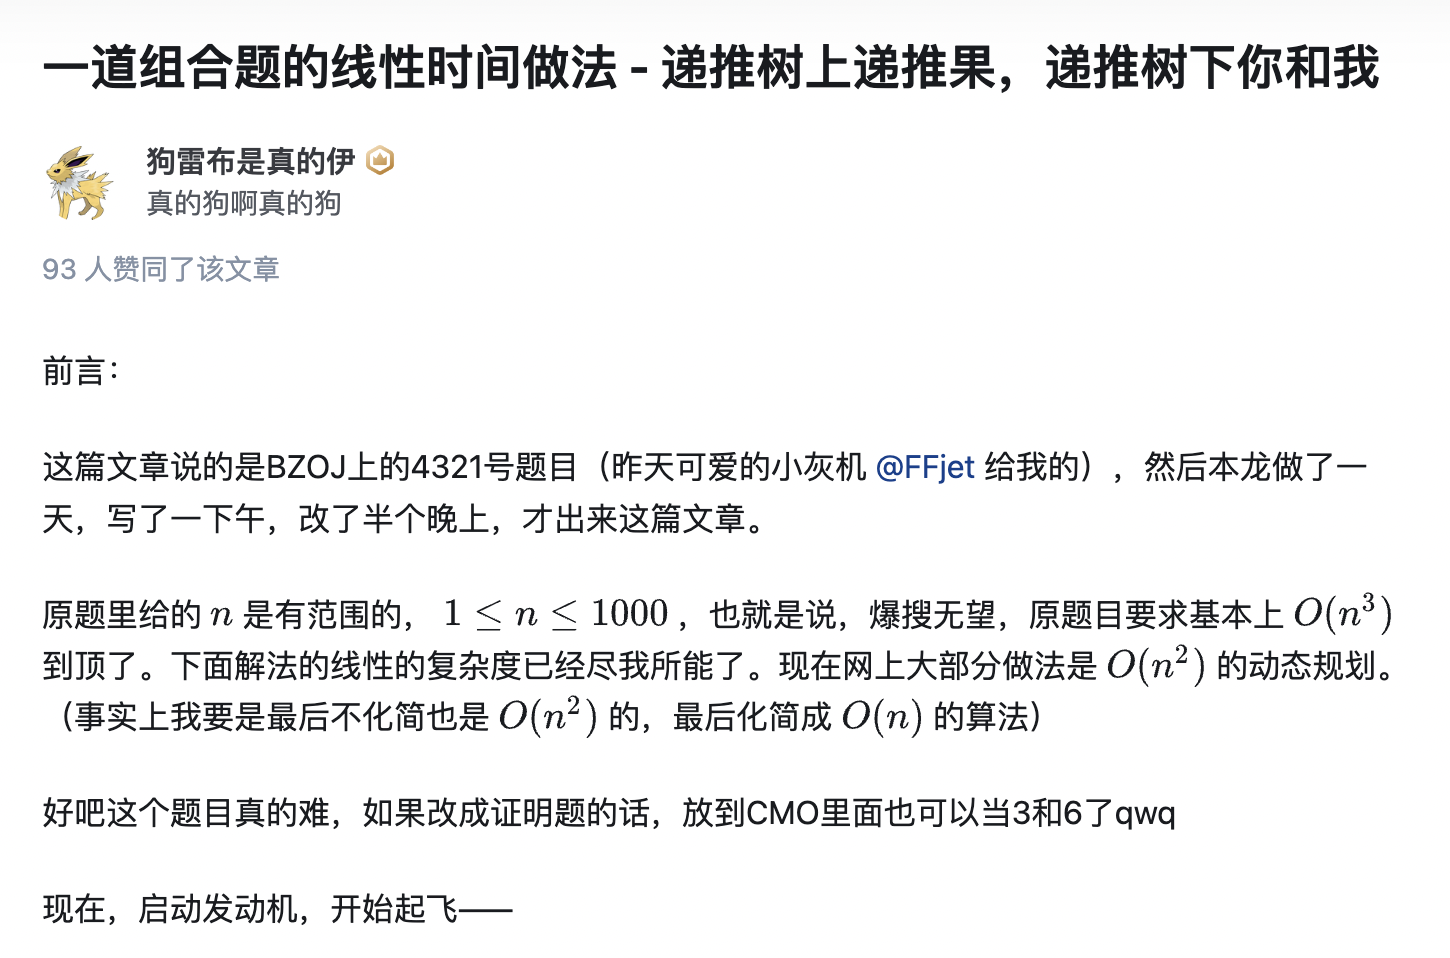
\includegraphics[scale=0.3]{zhihu.png}
    \url{https://zhuanlan.zhihu.com/p/56537011}
  \end{center}
  
  长达几页纸的双射... 有没有更简单的方法?
\end{frame}

\begin{frame}
  \frametitle{生成函数与递推式}

  对于相邻关系容斥, 可以写出生成函数
  \begin{align}
    \sum_n A_n x^n &= \left(\sum_{n=0}^\infty n! T^n\right) \circ \left( x - 2x^2 + 2x^3 - 2x^4 + 2x^5 + \cdots \right)\\
    &= \left(\sum_{n=0}^\infty n! T^n\right) \circ \left(x \frac {1-x}{1+x}\right).
  \end{align}

  \pause

  记 $S(T) = \sum_{n=0}^\infty n! T^n$, 将递推式 $S_n = nS_{n-1} + [n = 0]$ 转化为生成函数的微分方程
  \begin{align}
    S(T) &= 1 + (S(T) \cdot T)'\cdot T\\
    S &= 1 + TS + T^2S'.
  \end{align}

\end{frame}

\frame
{
  \begin{center}
    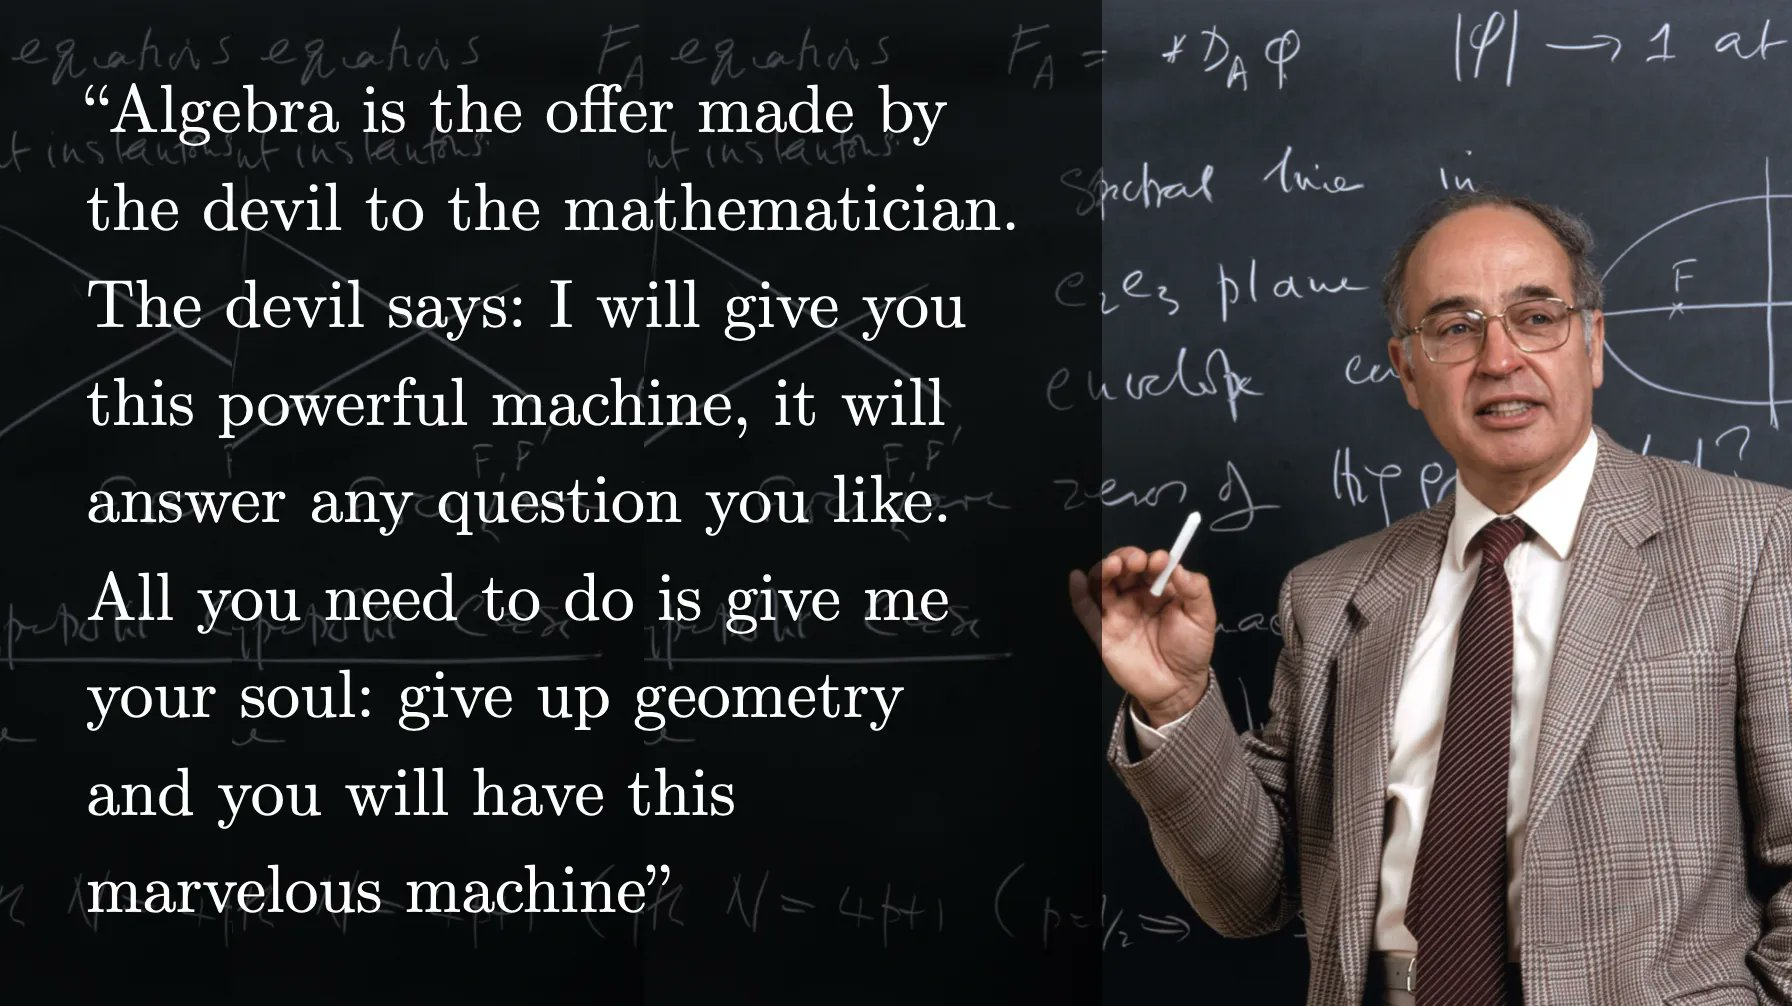
\includegraphics[scale=0.15]{Atiyah.jpeg}

    \hfill --- Michael Atiyah
  \end{center}
  \sout{生成函数是魔鬼和我们的交易. 魔鬼说: 我给你这个强大的机器, 它能回答任何你想问的问题.
  但是, 你必须付出代价, 你必须给我你的灵魂: 放弃组合意义, 然后你就能得到这台威力无穷的机器!}
}

\begin{frame}
  \frametitle{课间休息, 思考题}

  记 $\mathcal A$ 为 $2$-正则图构成的组合类, 证明其指数型生成函数是
  \begin{equation}
    A(x) = \exp \left( -\frac x 2 - \frac{x^2}{4} \right) \frac 1{\sqrt{1-x}}.
  \end{equation}

\end{frame}

\section{有关递推式的算法}

\frame
{
  \frametitle{生成函数 / 多项式 --- 算法}

  以下内容不会讲, 但是只假设它存在, 对后续内容的理解也基本没有影响.
  \begin{itemize}
    \item 快速 Fourier 变换: 高效计算 $A(x) B(x) \bmod x^n$.
    \item Newton 迭代法: 高效计算 $A(x)^{-1}$, $\log A(x)$, $\exp A(x)$ 等基本初等函数.
  \end{itemize}
  时间一般认为是 $\bigO(n\log n)$ 的, 但仔细思考计算模型会发现并不显然, 这里就记作 $\mathsf M(n)$.
}

\begin{frame}
  \frametitle{小故事: 整数乘法的长征}

  \begin{itemize}
    \item Колмого́ров 的猜测: $\mathsf M(N) = \Omega(N^2)$
  \end{itemize}
  \pause
    
  分治乘法!
  \begin{itemize}
    \item $\mathsf M(N) = \bigO\left(N^{\log 3 / \log 2}\right)$: \cnote{Karatsuba 1962}
  \end{itemize}
    \pause
  \begin{itemize}
    \item $\mathsf M(N) = N 2^{\bigO\left(\sqrt{\log N}\right)}$: \cnote{Toom 1963},
    \cnote{Sch\"onhage 1966}, \cnote{Knuth 1969}
  \end{itemize}
  \pause
    
  快速 Fourier 变换~{\bfseries \cnote{Gau\ss~1876}}, \cnote{Cooley--Tukey 1965}, 但单位根怎么存?
  \begin{itemize}
    \item $\mathsf M(N) = \bigO(N\log N \log \log N \log\log\log N \cdots)$: \cnote{Pollard 1971}
    \item $\mathsf M(N) = \bigO(N\log N \log \log N)$: {\bfseries\cnote{Sch\"onhage--Strassen 1971}}
    \includesvg[scale=0.15]{GMPLogo.svg}
    
    % 据说 $\stackrel{\text{GNU Multiple Precision}}{\text{\textcolor{red}{\bfseries GMP}}}$ 实现的就是此算法.
    \pause
    \item $\mathsf M(N) = N \log N 2^{\bigO(\log^* N)}$: \cnote{F\"urer 2007},
    \textcolor{teal}{\footnotesize Harvey},
    \textcolor{teal}{\footnotesize van der Hoeven}, 
    \textcolor{teal}{\footnotesize Lecerf}...
    \item $\mathsf M(N) = \bigO(N \log N)$: \cnote{Harvey--van der Hoeven 2019}
  \end{itemize}
  模型是多带 Turing 机, 可以大概理解成要衡量一个一个 bit 的操作.

  \pause
  \begin{itemize}
    \item 如果$\stackrel{\text{Network Coding Conjecture}}{\text{网\, 络\, 编\, 码\, 猜\, 想}}$成立, 那么这是不可改进的. \cnote{Afshani--Freksen--Kamma--Larsen 2019}
  \end{itemize}
\end{frame}

\subsection{半在线卷积的更快算法 --- 超越 ``CDQ 分治''}
\begin{frame}
  \frametitle{半在线卷积}

  \begin{itemize}
    \item<1-> 一般的卷积式
    \begin{equation}
      c_n = \sum_k a_k b_{n-k}
    \end{equation}
    也可以看做是一个递推式, 如果我们只有知道了 $c_n$ 才知道 $a_{n+1}, b_{n+1}$. 这是
    $\stackrel{\text{Relaxed Convolution}}{\text{在\, 线\, 卷\, 积}}$ 问题.
    \item<2-> 如果序列 $b$ 是一开始就完全知道的, 这是
    $\stackrel{\textbf{Semi }\text{Relaxed Convolution}}{\textbf{半\, }\text{在\, 线\, 卷\, 积}}$ 问题.
    \item<3-> 通过外层分治可以发现, 在线卷积并不比半在线卷积要难.
  \end{itemize}

\end{frame}

\begin{frame}
  \frametitle{半在线卷积的算法 \cnote{van der Hoeven 2002, 2007}}

  \begin{itemize}
    \item<1-> 直接的半在线卷积算法: 每次分治成两半, 递归求解, 时间复杂度 $\bigO(N\log^2 N)$.
    \item<2-> 每次分成 $B = \bigO(\log N)$ 块: 时间复杂度 $\bigO\left(\frac{N\log^2 N}{\log\log N}\right)$.
    \item<3-> 形如 $T(N) = 3 \sqrt N T(\sqrt N) + \bigO(N\log N)$ 的递归式:
    \begin{equation}
      \bigO\left(N(\log N)^{\log3/\log2}\right)
    \end{equation}
    \item<4-> 形如 $T(N) = 2\ell N^{1-1/\ell} T(N^{1/\ell}) + \bigO(\ell N\log N)$ 的递归式:
    \begin{equation}
      \bigO\left(N \log N \exp \left( 2\sqrt{\log 2 \log \log N} \right)\right)
    \end{equation}
    \item<5-> 没有平衡?
    \begin{equation}
      \mathsf{R}(n) = \bigO\left(N \log N \exp \left( \sqrt{2\log 2 \log \log N} \right) \sqrt{\log\log N} \right)
    \end{equation}
  \end{itemize}

\end{frame}

\subsection{线性递推的 Bostan--Mori 算法}
\begin{frame}
  \frametitle{线性递推的简洁算法 \cnote{Bostan--Mori 2021}}

  \begin{enumerate}
    \item<1-> 将生成函数写作 $P(x) / Q(x)$ 的形式
    \item<2-> 不妨分子分母同乘 $Q(-x)$, 得到 $P(x)Q(-x) / Q(x)Q(-x)$, 分母有什么特点?
    \item<3->  求第 $K$ 项的时间复杂度: $\bigO(\mathsf{M}(N)\log K)$. \textbf{只需要实现多项式乘法}.
  \end{enumerate}
\end{frame}

\subsection{多项式 Euclid 算法}

\begin{frame}
  \frametitle{多项式 Euclid}

  \begin{itemize}
    \item<1-> 给定多项式 $A(T), B(T)$, 求 $X(T), Y(T)$ 使得
    \begin{equation}
      AX + BY = \gcd(A, B).
    \end{equation}
    \item<2-> 说真的, 我们除了辗转相除法以外没有别的什么思路.
    \begin{align}
      A_0, & B_0\\
      A_1 = B_0, & B_1 = A_0 \bmod B_0\\
      A_2 = B_1, & B_2 = A_1 \bmod B_1\\
      & \dots \\
      A_\ell = B_{\ell - 1}, & B_\ell = A_{\ell - 1} \bmod B_{\ell - 1}
    \end{align}
  \end{itemize}

\end{frame}

\begin{frame}
  
  不妨设 $\deg A > \deg B$.
  \begin{align}
    A_0, & B_0\\
    A_1 = B_0, & B_1 = A_0 - B_0 \cdot Q_1\\
    A_2 = B_1, & B_2 = A_1 - B_1 \cdot Q_2\\
    & \dots \\
    A_\ell = B_{\ell - 1}, & B_\ell = A_{\ell - 1} - B_{\ell-1} \cdot Q_\ell,
  \end{align}
  
  \begin{itemize}
  %   \item 我们不妨写作
  %   \begin{equation}
  %     \begin{pmatrix}
  %       A_i \\ B_i
  %     \end{pmatrix} = \begin{pmatrix}
  %       0 & 1 \\ 1 & -Q_i
  %     \end{pmatrix} \begin{pmatrix}
  %       A_{i-1} \\ B_{i-1}
  %     \end{pmatrix}.
  %   \end{equation}
    \pause
    \item 如果有一个函数 $\textsc{HalfGCD}_N(A,B)$ 将两个次数 $< N$ 的多项式求出 $Q_1,\dots, Q_\ell$ 使得
    $\deg B_\ell < N/2$, 但 $\deg A_\ell \geq N/2$...
    \pause
    \item 那么调用 $\log N$ 次就可以得到完整的 Euclid 过程商的序列, 而且复杂度可以被主定理控制.
  \end{itemize}

\end{frame}

\begin{frame}
  \frametitle{折半 Euclid 算法 \cnote{Knuth 1970} \cnote{Sch\"onhage 1971} \cnote{Moenck 1973}}

  不妨设 $N$ 是 $2$ 的幂, $\deg A > \deg B$.

  \begin{itemize}
    \item<1-> 函数 $\textsc{HalfGCD}_N(A,B)$ 的目的: 将两个次数 $< N$ 的多项式求出 $Q_1,\dots, Q_\ell$ 使得
    $\deg B_\ell < N/2$, 但 $\deg A_\ell \geq N/2$.
    \item<2-> \textbf{前期的计算不会影响太低位:} $\deg (Q_1 \cdots Q_\ell) = \deg A_0 - \deg A_\ell < N/2$.
    \item<3-> 如果对于 $A = T^L A' + O(T^{L-1})$, $B = T^L B' + O(T^{L-1})$ 做
    $\textsc{HalfGCD}_{N/2}(A', B')$...
    \item<4-> 由于我们可以写成矩阵,
    \begin{equation}
      A_i = B_{i - 1}, B_i = A_{i - 1} - B_{i-1} \cdot Q_i
      \iff
      \begin{pmatrix}
        A_i \\ B_i
      \end{pmatrix} = \begin{pmatrix}
        0 & 1 \\ 1 & -Q_i
      \end{pmatrix} \begin{pmatrix}
        A_{i-1} \\ B_{i-1}
      \end{pmatrix}.
    \end{equation}
    \item<4-> 有
    \begin{equation}
      \begin{pmatrix}
        0 & 1 \\ 1 & -Q_\ell
      \end{pmatrix} \cdots \begin{pmatrix}
        0 & 1 \\ 1 & -Q_1
      \end{pmatrix} 
      \begin{pmatrix}
        A\\ B
      \end{pmatrix}
      = T^L\begin{pmatrix}
        A' \\ B'
      \end{pmatrix} + O(T^{L-1}) \cdot O(T^{N/4 - 1}).
    \end{equation}
  \end{itemize}

\end{frame}

\begin{frame}
  \frametitle{折半 Euclid 算法 \cnote{Knuth 1970} \cnote{Sch\"onhage 1971} \cnote{Moenck 1973}}

  \begin{itemize}
    \item<1-> 如果对于 $A = T^L A' + O(T^{L-1})$, $B = T^L B' + O(T^{L-1})$ 做
    $\textsc{HalfGCD}_{N/2}(A', B')$, 有
    \begin{equation}
      \begin{pmatrix}
        0 & 1 \\ 1 & -Q_\ell
      \end{pmatrix} \cdots \begin{pmatrix}
        0 & 1 \\ 1 & -Q_1
      \end{pmatrix} 
      \begin{pmatrix}
        A\\ B
      \end{pmatrix}
      = T^L\begin{pmatrix}
        A' \\ B'
      \end{pmatrix} + O(T^{L-1}) \cdot O(T^{N/4 - 1}).
    \end{equation}
    \item<2-> 第一次取 $L = N/2$, 将 $(A, B)$ 约化到 $\deg A \geq \nicefrac{3}{4} N > \deg B$,
    然后做一次取模.
    \item<3-> 第二次取 $L = N/4$, 将 $(A, B)$ 约化到 $\deg A \geq \nicefrac{1}{2} N > \deg B$.
    \item<4-> 这总共调用了两次分治, 有
    \begin{equation}
      T(N) = 2T(N/2) + \bigO(\mathsf M(N)),
    \end{equation}
    解得 $T(N) = \bigO(\mathsf{M}(N) \log N)$.
  \end{itemize}

\end{frame}

\begin{frame}
  \frametitle{连分式展开}

  我们求出的序列的一种直观解释:

  \begin{align}
    \frac A B &= Q_1 + \frac{A\bmod B}{B}\\
    &= Q_1 + \frac 1{B / (A \bmod B)}\\
    &= Q_1 + \frac 1{Q_2 + \frac 1{Q_3 + \ddots}}\\
    &:= [Q_1; Q_2,\dots, Q_\ell].
  \end{align}

\end{frame}

\begin{frame}
  \frametitle{线性递推式重建}

  \begin{itemize}
    \item<1-> 已知一个 $\leq N$ 阶线性递推式的前 $2N$ 项 $a_0,\dots,a_{2N-1}$, 求递推式.
    \item<2-> 我们知道, 这是要找 $P, Q$ 满足 $A \equiv P/Q \pmod {x^{2N}}$, 且 $\deg P < N, \deg Q \leq N$.
  \end{itemize}
  \onslide<3->{
    \begin{definition}[Pad\'e 逼近]
      给定 $A(x)$, 求 $\deg P \leq N_1$, $\deg Q \leq N_2$ 满足
      \begin{equation}
        P - AQ \equiv 0 \pmod {x^{N_1+N_2+1}}.
      \end{equation}
    \end{definition}
  }
  \onslide<4->{
    \begin{definition}[有理函数重建]
      给定 $A(x)$ 和模 $M(x)$, 求 $\deg P \leq N_1$, $\deg Q \leq N_2$ 满足
      \begin{equation}
        P - AQ \equiv 0 \pmod {M},
      \end{equation}
      其中 $\deg M = N_1 + N_2 + 1$.
    \end{definition}
  }

\end{frame}

\begin{frame}
  \frametitle{连分式展开 $\implies$ 有理函数重建}

  \begin{definition}[有理函数重建]
    给定 $A(x)$ 和模 $M(x)$, 求 $\deg P \leq N_1$, $\deg Q \leq N_2$ 满足
    \only<1>{
      \begin{equation}
        P - AQ \equiv 0 \pmod {M},
      \end{equation}
    }\only<2->{
      \begin{equation}
        P = AQ + BM,
      \end{equation}
    }
    其中 $\deg M = N_1 + N_2 + 1$.
  \end{definition}
  \onslide<3->{
  \begin{align}
    A_0 &= M \\
    \only<3>{\makebox[0pt][l]{\makebox[\widthof{$\overbracket{A_1}^{\deg < \deg A_0}$}][c]{$A_1$}}
    \phantom{\overbracket{A_1}^{\deg < \deg A_0}}}
    \only<4>{\overbracket{A_1}^{\deg < \deg A_0}}
    &= A  & \onslide<4> {= O(x^{\deg A_0 - \deg A_0}) \bm{\cdot} (M, A)} \\
    \only<3>{\makebox[0pt][l]{\makebox[\widthof{$\overbracket{A_2}^{\deg < \deg A_1}$}][c]{$A_2$}}
    \phantom{\overbracket{A_2}^{\deg < \deg A_1}}}
    \only<4>{\overbracket{A_2}^{\deg < \deg A_1}}
     &= A_0 - A_1 \cdot Q_1 & \onslide<4>{ = O(x^{\deg A_0 - \deg A_1}) \bm{\cdot} (M, A)} \\
    &\dots
  \end{align}
  }

\end{frame}

\frame
{
  \frametitle{间奏: 纠错码的快速算法}

  纠错码是通信的基础, 考虑固定的一个有限的字符集 $\Sigma$,
  一个\textbf{纠错码}可以看做一个函数 $C\colon \Sigma^n\to \Sigma^m$ ($m\geq n$).

  所以为了保证纠错码的可靠性, 我们关心``距离'':
  \begin{equation}
    d = \min_{\substack{x,y\in \Sigma^n\\x\neq y}} \delta(C(x), C(y)),
  \end{equation}
  其中 $\delta$ 是 $\Sigma^m$ 上的 Hamming 距离. 易见, 如果传输中错误的字符数量
  $< d/2$, 那么我们可以完美地恢复原来的信息.
}

\frame
{
  \frametitle{基于多项式求值的编码 \cnote{Reed--Solomon 1960}}

  令字符集为有限域 $\bbF$ 满足 $|\bbF| \geq m$, 令 $\alpha_1,\dots, \alpha_m$
  是 $\bbF$ 的 $m$ 个不同的元素, 考虑如下的映射:
  \begin{equation}
    C(a_0,\dots, a_{n-1}) \mapsto \left( \sum_{j=0}^{n-1} a_j \alpha_i^j \right)_{i=1}^m,
  \end{equation}
  也即将信息 $a_0,\dots, a_{n-1}$ 看做一个 $n-1$ 次多项式 $f(x) = \sum_{j=0}^{n-1} a_j x^j$,
  在 $m$ 个给定点处的取值.

  注意到 $n$ 个点值就足够确定一个 $n-1$ 次多项式, 所以 \textbf{Reed--Solomon 码}的距离满足 $d \geq m-n+1$.
}


\frame
{
  \frametitle{Reed--Solomon 编码的快速纠错 \cnote{Berlekamp--Welch 1986}}

  给一个 $n-1$ 次多项式 $f(x)$, 如果 $f(\alpha_1),\dots,f(\alpha_m)$ 中有 $\leq (m-n)/2$ 个错误, 一定
  可以唯一地还原出 $f$ 的系数, 但是如何快速计算?

  \bigskip

  不妨设给定的 $y_1,\dots,y_m$ 确定出来的多项式是 $g(x)$, 那么 $g(x) - f(x)$ 只在 $\beta_1,\dots,\beta_k$
  上非零, 所以
  \begin{equation}
    (g(x) - f(x))(x-\beta_1)\cdots(x-\beta_k) \equiv 0 \pmod {(x-\alpha_1)\cdots(x-\alpha_m)},
  \end{equation}
  注意写作 $r(x) = (x-\beta_1)\cdots(x-\beta_k)$, 那么
  \begin{equation}
    \deg r + \deg (f \cdot r) = k + (n-1+k) \leq m-1,
  \end{equation}
  可以考虑直接对 $g(x)$ 进行有理函数重建.
}

\subsection{Hermite--Pad\'e 逼近}

\begin{frame}
  \frametitle{更加一般的问题}

  \onslide<1->{
    \begin{definition}[Hermite--Pad\'e 逼近]
      给定多项式 $A_1,\dots, A_m$ 和度数限制 $d_1,\dots, d_m$, 求 $P_1,\dots,P_m$ 使得
      \begin{itemize}
        \item $\deg P_i < d_i$,
        \item $P_1 A_1 + \cdots + P_m A_m \equiv 0 \pmod {x^{d_1 + \cdots + d_m - 1}}$.
      \end{itemize}
    \end{definition}
  }

  \begin{itemize}
    \item<2-> $\stackrel{\text{Min25 \quad BM}}{\text{找寻整式递推式}}$可以直接对 $(A, A', \dots, A^{(m-1)})$ 调用 Hermite--Pad\'e 逼近的算法.
    \item<2-> 找寻最小多项式可以直接对 $(1, A, \dots, A^{m-1})$ 调用 Hermite--Pad\'e 逼近的算法.
    \item<3-> 记 $\sigma = d_1 + \cdots + d_m - 1$, Hermite--Pad\'e 逼近的时间复杂度可以在 $\widetilde \bigO(m^{\omega - 1} \sigma)$
    的时间内完成, 其中 $\omega$ 是矩阵乘法的指数\footnote<3->{现在 $\omega\leq 2.371552$. \cnote[\tiny]{Williams--Xu--Xu--Zhou 2023}}. \cnote{Labahn--Zhou 2012}
  \end{itemize}

\end{frame}

\begin{frame}
  \frametitle{解 Toeplitz 方程}

  \begin{definition}[Toeplitz 矩阵]
    形如 $(a_{i-j})_{i,j}$ 的矩阵, 其中 $a$ 是下标从 $-(N-1)$ 到 $N-1$ 的数列.
  \end{definition}

  \begin{itemize}
    \item<2-> Toeplitz 方程可以写作
    \begin{equation}
      a(T) \cdot x(T) = b(T) + \Omega(T^{N-2}) + O(T^{2N-1}),
    \end{equation}
    \item<3-> 转化成
    \begin{equation}
      a(T) \cdot \underbracket{x(T)}_{\deg < N} - b(T) \cdot \underbracket{1}_{\deg < 1}
      - 1 \cdot \underbracket{r(T)}_{\deg < N - 1} \equiv 0 \pmod {T^{2N-1}}.
    \end{equation}
    \item<4-> 刚好 $N + 1 + (N - 1) - 1 = 2N-1$, 符合 Hermite--Pad\'e 逼近的形式.
  \end{itemize}

\end{frame}

\begin{frame}
  \frametitle{解的多项式基}

  \begin{itemize}
    \item 给定 $\bm{A} \in \bbF \llbracket x \rrbracket^m$, 定义 $V_s = \{ \bm{P} \in \bbF[x]^m :
    \bm{P \cdot A} \equiv 0 \pmod {x^s} \}$.
    \item 记 $\deg (\bm{P}) = \max_{1\leq i \leq m} \{ \deg (\bm{P}_i) \}$, $\type (\bm{P})$ 为取到最大值的最大的 $i$.
    \item $V_s$ 的~\textbf{极小基}: 对每个 $i$, 选取 $\bm{Q}_i$ 是 $\type(\bm P) = i$ 中度数
    最小的一个.
  \end{itemize}
  性质:
  \begin{itemize}
    \item<2-> 确实是基: $\bm{Q}_1,\dots,\bm{Q}_m$ 可以组合出 $V_s$ 中的元素.
    \item<3-> 最优性: $V_{md - 1}$ 的一组极小基中, 次数最小的 $\bm{Q}_i$ 是 $\deg < d$ 的 Hermite--Pad\'e 逼近的形式
    的一组解.
  \end{itemize}

\end{frame}

\begin{frame}
  \frametitle{极小基的维护}

  \begin{itemize}
    \item 按照 $s$ 从小到大的顺序逐渐维护 $V_s$ 的一组极小基.
    \item $V_0$ 是平凡情况, 有 $\bm{Q}_{i j} = [i = j]$.
    \item 从 $V_s$ 推到 $V_{s+1}$ 的极小基 $\{ \widetilde {\bm{Q}}_{i} \}$:
    \begin{itemize}
      \item<2-> 如果 $x^{s+1} \mid\bm{Q}_i \bm{\cdot A}$, 可以直接保留, $\widetilde {\bm{Q}}_{i} = \bm{Q}_i$.
      \item<3-> 否则存在 $x^s$ 次项, 设 $\ell$ 是这种情况的 $i$ 中按照 $(\deg, \type)$ 的字典序比较下最小的那个.
      \item<4-> 对于这样的 $i \neq \ell$, 通过 $\widetilde{\bm{Q}}_i = \bm{Q}_i - \lambda \cdot \bm{Q}_\ell$
      消去 $x^s$ 次项 (为什么 $\type (\widetilde{\bm{Q}}_i) = i$?)
      \item<5-> 对于 $\ell$, 必须有 $\widetilde{\bm{Q}}_\ell = x\cdot \bm{Q}_\ell$. (总得牺牲一个)
    \end{itemize}
    \item<6-> 正确性: 考虑消元.
    \item<7-> 时间复杂度: $\bigO(m^3 d^2) = \bigO(m \sigma^2)$. \cnote{Derksen 1994}
    \item<8-> 改进成一般情况: 把 $\deg$ 的定义改为 $\deg (\bm P) = \max_i \{ \deg (\bm{P}_i) - d_i \}$.
    \item<9-> 改进复杂度: 将 HalfGCD 的思想应用到上述过程!
  \end{itemize}

\end{frame}

\begin{frame}
  \frametitle{大炮现状}

  \begin{definition}[Hermite 标准型]
    任何一个多项式矩阵 $\bm{A} \in \bbF[x]^{m\times m}$, 存在 $\bm{H} = \bm{AU}$ ($\det (\bm{U}) \in \bbF^\times$) 使得
    \begin{itemize}
      \item $\bm{H}$ 是下三角矩阵.
      \item $\deg(\bm{H}_{ij}) < \deg (\bm{H}_{ii})$.
    \end{itemize}
  \end{definition}
  \begin{itemize}
    \item 在 $\widetilde \bigO( m^{\omega} \deg (\bm{A}) )$ 时间内计算 Hermite 标准型和 $\det(\bm A)$.
    ($\deg (\bm{A})$ 是``平均次数''!)
    \cnote{Labahn--Neiger--Zhou 2012}
    \item Popov 标准型, $\bm{s}$-约化型, ...
    \item Hermite--Pad\'e 逼近, 但是从 $\bmod x^\sigma$ 改成 $\bmod M(x)$.
    \item 多项式矩阵的 ``gcd''.
    \item ...
  \end{itemize}
  很多算法在 \includesvg[scale=0.2]{Sage-logo-2018.svg} 中有实现.

\end{frame}

\begin{frame}
  \frametitle{延伸阅读}

  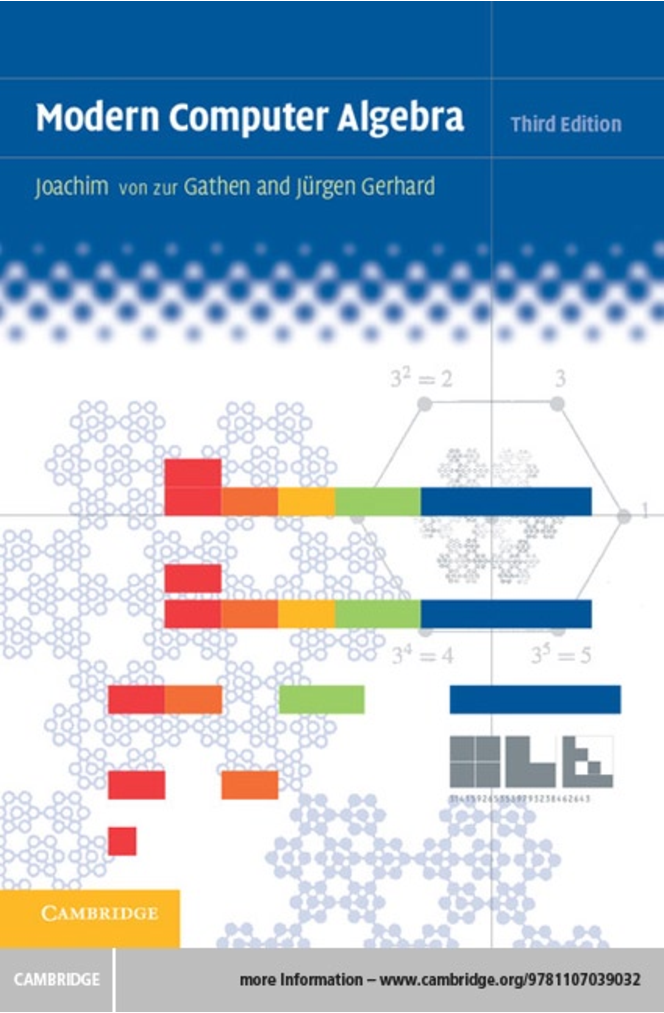
\includegraphics[scale=0.3]{GG.pdf}
  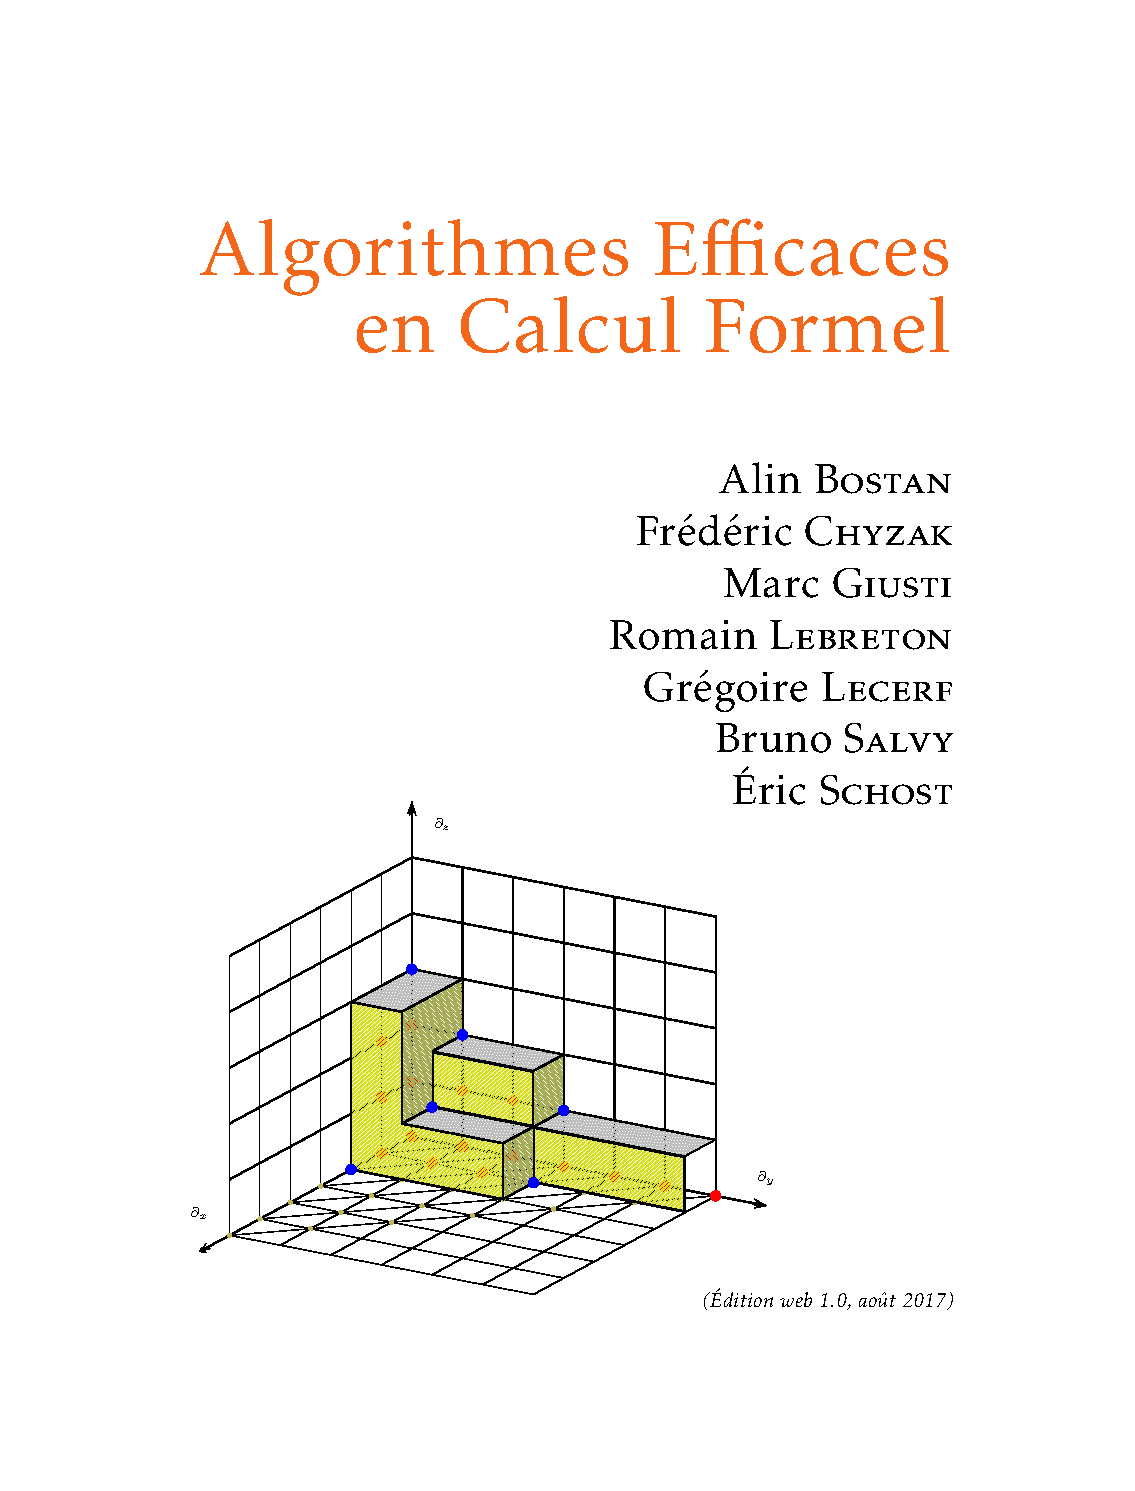
\includegraphics[scale=0.25]{AECF.pdf}

  \begin{itemize}
    \item von zur Gathen \& Gerhard: 经典之作.
    \item AECF: 成书时间较新, 有网络版, 但是是法语.
  \end{itemize}

\end{frame}

\section{整式递推的理论}

\begin{frame}
  \frametitle{定义}

  \begin{definition}[整式递推]
    对于一个数列 $\{a_n\}_{n\geq 0}$, 我们称其为
    $\stackrel{\text{P-Recursive}}{\textbf{整式递推}}$ 的, 当且仅当存在多项式
    $p_0(x), p_1(x), \dots, p_m(x)$ 使得, 对于 $n\geq m$, 有
    \begin{equation}
      p_0(n) a_n + p_1(n) a_{n-1} + \cdots + p_m(n) a_{n-m} = 0.
    \end{equation}
  \end{definition}
  \pause
  \begin{definition}[微分有限]
    对于一个生成函数 $A(x)$, 我们称其为$\stackrel{\text{D-Finite}}{\textbf{微分有限}}$的, 当且仅当存在多项式 $f_0(x),\dots,f_m(x)$, 有
    \begin{equation}
      f_0(x) A(x) + f_1(x) A'(x) + \cdots + f_m(x) A^{(m)}(x) = 0.
    \end{equation}
  \end{definition}
  \pause
  \textbf{定理:} $\{a_n\}$ 整式递推 $\iff A(x)$ 微分有限.

\end{frame}

\subsection{为什么要研究整式递推}

\begin{frame}
  \frametitle{为什么要研究整式递推?}

  \begin{itemize}
    \item 大量的组合计数问题的数列最终都被发现是整式递推的.
    \pause
    \item 以 $k$-正则图计数为例.
    \item 之前的思考题里提到了, $k=2$ 的时候生成函数形如
    \begin{equation}
      A(x) = \exp \left( -\frac x 2 - \frac{x^2}{4} \right) \frac 1{\sqrt{1-x}},
    \end{equation}
    \item 微分有限的生成函数关于各种运算 \textbf{具有良好的封闭性}, 我们之后会看到有办法直接证明上述序列是整式递推的.
    \pause
    \item 随后, $k=3$ 和 $k=4$ 的情况也被证明是整式递推的, 这一方法并非出于对于正则图组合结构的归纳. \cnote{Goulden--Jackson 1986}
    \item 之后, 任意 $k$ 的情况也被证明. \cnote{Gessel 1990} 他们的证明方法源于发展了~\textbf{无穷元对称微分有限生成函数}~的理论.
  \end{itemize}

\end{frame}

\subsection{线性空间的表述方式}

\begin{frame}
  \frametitle{线性代数 101}

  \begin{itemize}
    \item 域 $\bbF$ 上的一个线性空间 $V$ 是一个集合, 配备加法和对 $\bbF$ 的数乘运算, 满足线性性
    ($\alpha, \beta \in \bbF$, $u, v \in V$):
    \begin{itemize}
      \item $\alpha \cdot (u + v) = \alpha \cdot u + \alpha \cdot v$,
      \item $(\alpha + \beta) \cdot u = \alpha \cdot u + \beta \cdot v$,
      \item $\alpha \cdot (\beta \cdot v) = (\alpha \beta) \cdot v$.
    \end{itemize}
    \item 我们会用到的线性空间: 多项式 $\bbF[x]$, 形式幂级数 $\bbF \llbracket x \rrbracket$,
    形式 Laurent 级数 $\bbF \llparenthesis x \rrparenthesis$, 数列 $\bbF^{\bbZ_{\geq 0}}$, ...
    \item 线性变换 $T \colon V \to W$ 是一个函数, 保持线性性:
    \begin{itemize}
      \item $T(u + \alpha v) = Tu + \alpha Tv$.
    \end{itemize}
    \item 我们关心的运算 $\partial$ 在 $\bbF[x]$, $\bbF \llbracket x \rrbracket$ 和 $\bbF \llparenthesis x \rrparenthesis$
    都是 $\bbF$-线性的.
    \item 每个线性空间都有个维数, 是它的基的大小, 如果基的大小是有限的, 称是有限维线性空间 ($\dim V = n < \infty$).
    \item 比如 $\bbF[x]$ 不是有限维的, $\bbF^n$ 是 $n$ 维的, 次数 $\leq n$ 的多项式是 $n+1$ 维的.
  \end{itemize}

\end{frame}

\begin{frame}
  \frametitle{微分有限的线性空间表述}

  \begin{itemize}
    \item 有理分式 $\bbF(x)$ 由于可以做除法, 所以它是个域.
    \item $\bbF\llparenthesis x \rrparenthesis$ 不仅是 $\bbF$-线性空间, 还具有 $\bbF(x)$-线性结构!
    \begin{itemize}
      \item 商 $\bbF[x]^{-1}\bbF\llbracket x\rrbracket \hookrightarrow \bbF\llparenthesis x \rrparenthesis$ 
      容易识别, 这一嵌入进一步是同构, 但在多元情况并不典范.
    \end{itemize}
    \begin{definition}[微分有限]
      一个生成函数 $F(x)$ 是~\textbf{微分有限}~的当且仅当
      \begin{equation}
        \calD F := \Span_{\bbF(x)} \left\{ \partial^k F : k \in \bbZ_{\geq 0} \right\}
      \end{equation}
      是有限维 $\bbF(x)$-线性空间.
    \end{definition}
    \item 这和我们之前的定义等价, 但更容易推广到多元情况.
  \end{itemize}

\end{frame}

\begin{frame}
  \frametitle{微分有限的基本性质}

  \begin{theorem}
    若 $F(x), G(x)$ 微分有限, 则 $F+G$ 微分有限.
  \end{theorem}
  \begin{proof}
    令 $\{\alpha_1,\dots,\alpha_n\}$ 为 $\calD F$ 的基, $\{\beta_1,\dots,\beta_m\}$ 为 $\calD G$ 的基, 那么
    \begin{equation}
      \partial^k (F+G) = \partial^k F + \partial^k G = \sum a_i \alpha_i + \sum b_i \beta_i.
    \end{equation}
    故 $\dim_{\bbF(x)} \calD(F+G) \leq n+m < \infty$.
  \end{proof}

\end{frame}

\begin{frame}
  \frametitle{微分有限的基本性质}

  \begin{theorem}
    若 $F(x), G(x)$ 微分有限, 则 $FG$ 微分有限.
  \end{theorem}
  \begin{proof}
    令 $\{\alpha_1,\dots,\alpha_n\}$ 为 $\calD F$ 的基, $\{\beta_1,\dots,\beta_m\}$ 为 $\calD G$ 的基, 那么
    $\partial^k(FG)$ 被 $\partial^i F \partial^j G$ 线性表出, 因此被 $\{\alpha_i \beta_j\}$ 线性表出.
    
    故 $\dim_{\bbF(x)} \calD(FG) \leq nm < \infty$.
  \end{proof}

\end{frame}

\begin{frame}
  \frametitle{微分有限的基本性质}

  \begin{theorem}
    若 $F(x), G(x)$ 微分有限, 则 $F+G$ 微分有限.
  \end{theorem}
  \begin{theorem}
    若 $F(x), G(x)$ 微分有限, 则 $FG$ 微分有限.
  \end{theorem}
  \begin{itemize}
    \item 如何在计算上得到之前定义的对应的方程?
    \pause
    \item $F/G$ 并不一定是微分有限的:
    \begin{equation}
      \frac{x}{\exp x - 1}.
    \end{equation}
  \end{itemize}

\end{frame}

% \begin{frame}
%   \frametitle{整式递推的线性空间表述}

%   生成函数天生可以做除法, 数列除以多项式 $p(n)$ 会有微妙的问题.

%   \begin{definition}[芽]
%     两个序列 $\{a_n\}, \{b_n\}$, 我们称 $a\sim b$ 当且仅当 $a_n = b_n$ 对于充分大的 $n$ 皆成立.

%     这给出一个 $\bbF^{\bbZ_{\geq 0}}$ 上的等价关系, 我们称一个等价类 $\widetilde a$ 为一个 $\stackrel{\text{germ}}{\text{芽}}$.
    
%     记为 $\mathcal J_\bbF = \bbF^{\bbZ_{\geq 0}}/\sim$.
%   \end{definition}
%   \begin{itemize}
%     \item 如果要除以一个多项式 $p(n)$, 由于多项式只有有限个零点, 总能找到 $\{b_n\}$ 使得
%     $\widetilde{ \{b_n\cdot p(n)\} } = \widetilde{ \{a_n\} }$, 这就定义出了
%     $\widetilde a / p(n)$, 给出了 $p(x) / q(x)$ 对 $\mathcal J_\bbF$ 的作用
%     \begin{equation}
%       a_n \mapsto \frac{p(n)}{q(n)} a_n.
%     \end{equation}
%   \end{itemize}

% \end{frame}

% \begin{frame}
%   \frametitle{整式递推的基本性质}

%   定义平移算子
%   \begin{equation}
%     \rmT \{a_n\} = \{a_{n+1}\}.
%   \end{equation}

%   \begin{definition}[整式递推]
%     对于 $\widetilde a \in \mathcal J_\bbF$, 我们称其为~\textbf{整式递推}~的当且仅当
%     \begin{equation}
%       \Span_{\bbF(x)} \widetilde a \left\{ \rmT^k \widetilde a : k \in \bbZ_{\geq 0} \right\}
%     \end{equation}
%     是有限维 $\bbF(x)$-线性空间.
%   \end{definition}
  
%   \begin{theorem}
%     若 $\{a_n\}, \{b_n\}$ 整式递推, 则 $\{a_n b_n\}$ 整式递推.
%   \end{theorem}
%   转换到对于芽 $\mathcal J_\bbF$ 上进行证明, 和微分有限的情况如出一辙.

% \end{frame}


\begin{frame}
  \frametitle{作为一个关心计算的人, 我为什么要研究整式递推?}

  \begin{itemize}
    \item $\partial$ 连同四则运算, 很大程度上勾勒了我们有哪些工具计算一个序列.
    \item 生成函数的层级:
    \begin{center}
      $\text{有理} \quad \subset \quad \text{代数} \quad \subset \quad \text{微分有限} \quad
      \subset \quad \stackrel{\text{D-Algebraic}}{\text{微分代数}} \quad \subset \quad \bbF \llbracket x \rrbracket$
    \end{center}
    \pause
    \begin{itemize}
      \item 如果是有理函数, 我们可以 $O(\log N)$ 就计算出第 $N$ 项, 相当快速.
      \item 如果微分有限, 我们可以 $O(\mathsf M(\sqrt N))$ 就计算出第 $N$ 项
      \cnote{Chudnovsky--Chudnovsky 1988} \cnote{Bostan--Gaudry--Schost 2007}, 或者 $O(N)$ 计算出前 $N$ 项.
      \item 如果微分代数, 我们至少可以用半在线卷积的方法 $O(\mathsf R(N))$ 计算出前 $N$ 项.
    \end{itemize}
  \end{itemize}

\end{frame}

\begin{frame}
  \frametitle{题外话: 疑难数列之整数拆分}

  \begin{itemize}
    \item 整数拆分的生成函数
    \begin{equation}
      F(x) = \prod_{n=1}^\infty \frac 1{1-x^n},
    \end{equation}
    \pause
    看起来应该是非常困难的序列, 但它居然~\textbf{是}~微分代数的!
    \begin{multline}
      4F^3 F'' + 5x F^3 F''' + x^2 F^3 F^{(4)} - 16F^2 F'^2  - 15x F^2 F' F'' + 20x^2 F^2 F' F'''\\
       - 39x^2 F^2 F''^2 + 10x F F'^3  + 12x^2 F F'^2 F'' + 6x^2 F'^4 = 0.
    \end{multline}
    \pause
    \item 深层原因或许要涉及 $\stackrel{\text{Modular Form}}{\text{模形式}}$, 这是现代数学的重要分支之一, 远远
    超出了本次讲故事的狩猎范围.
  \end{itemize}

\end{frame}

\begin{frame}
  \frametitle{题外话: 疑难数列之禁子结构排列}

  \begin{itemize}
    \item 给定一个有限个排列构成的集合 $\mathcal F$, 记 $\mathsf A_n(\mathcal F)$ 是所有没有出现过
    $\mathcal F$ 中结构的 $n$ 阶排列的数量.
    \pause
    \item 例如 $\mathsf A_n(\{123\})$ 就是 Catalan 数 $C_n$.
    \pause
    \item 但到了形态有 $4$ 阶排列, 就已经出现了没法解决的问题了, 例如 $\mathsf A_n(\{1324\})$.
    \begin{itemize}
      \pause
      \item 人们现在~\textbf{不知道}~如何在多项式时间内计算 $\mathsf A_n(\{1324\})$. 
      尽管人们现在已经确认计算 $\mathsf A_n(\mathcal F)$ \textbf{很可能}是困难的.
      (如果存在多项式时间算法计算 $\mathsf A_n(\mathcal F)\bmod 2$, 那么 $\EXP = \parity\EXP$.
      \cnote{Garrabrant--Pak 2015})
      \pause
      \item 人们现在~\textbf{不知道}~如何证明 $\mathsf A_n(\{1324\})$ 并非整式递推.
      尽管已经知道存在 $\mathcal F \subset \mathfrak S_{80}$ 使得 $\mathsf A_n(\mathcal F)$ 不是整式递推.
      \cnote{Garrabrant--Pak 2015}
      \pause
      \item 人们现在甚至不能证明 $\mathsf A_n(\{1324\})$ 的渐进行为, 只能根据 $n\leq 50$ 的数值结果做出猜测:
      \cnote{Conway--Guttmann--Zinn-Justin 2017}
      \begin{equation}
        \mathsf A_n(\{1324\}) \sim C \cdot \lambda^n \mu^{\sqrt n} n^\alpha.
      \end{equation}
    \end{itemize}
  \end{itemize}

\end{frame}

\subsection{代数幂级数}

\begin{frame}
  \frametitle{代数幂级数}

  \begin{definition}[代数幂级数]
    $F(x)\in \mathbb F\llparenthesis x\rrparenthesis$ 是~\textbf{代数}~的当且仅当有多项式方程 $P\in \bbF[X, T]$ 满足
    \begin{equation}
      P(x, F) = 0.
    \end{equation}
  \end{definition}
  代数幂级数关于除法是封闭的!
  \begin{theorem}
    代数幂级数构成域, 也即 $F + G, F G, F/G$ 都是代数幂级数.
  \end{theorem}
  加法和乘法略去, 仅勾勒除法的封闭性.
  \begin{proof}
    如果 $P(x, F) = 0$, 写作 $P(X, T) = \prod_\alpha (T - \alpha(x))$, 那么
    \begin{equation}
      \prod_\alpha (T - 1/\alpha) = 0 \implies 
      \prod_\alpha (\alpha T - 1) = 0 \implies
      T^{\deg P} P(x, 1/T) = 0. \qedhere
    \end{equation}
  \end{proof}

\end{frame}

\begin{frame}
  \frametitle{代数幂级数的微分有限性}

  \begin{theorem}
    如果 $u(x)$ 是代数的, 那么它是微分有限的.
  \end{theorem}
  \begin{proof}[证明 (勾勒)]
    设 $u$ 满足一个次数为 $n$ 的代数方程 $P(x, u) = 0$, 求导可以得到
    $\calD u \subset \Span_{\bbF(x)} \{ u^k : 0\leq k < n \}$.
  \end{proof}
  后者其实就是代数扩张 $\mathbb K := \bbF(x)(u)$.

  \begin{theorem}
    如果 $F(x)$ 是微分有限的, $u(x)$ 是代数的, 那么 $F(u(x))$ 是微分有限的.
  \end{theorem}
  \begin{proof}[证明 (勾勒)]
    只需证明 $\partial^k (F\circ u)$ 张成的
    是有限维 $\mathbb K$-空间.
  \end{proof}

\end{frame}

\begin{frame}
  \frametitle{大炮开火!}

  \begin{itemize}
    \item $2$-正则图构成的组合类, 其指数型生成函数是
    \begin{equation}
      A(x) = \exp \left( -\frac x 2 - \frac{x^2}{4} \right) \frac 1{\sqrt{1-x}}.
    \end{equation}
    \pause
    \item $\exp \left( -\frac x 2 - \frac{x^2}{4} \right)$ 是微分有限的, 因为
    \pause
    \begin{itemize}
      \item $\exp x$ 是微分有限的.
      \pause
      \item $-\frac x 2 - \frac{x^2}{4}$ 是有理的, 所以是代数的.
    \end{itemize}
    \pause
    \item $\frac 1{\sqrt{1-x}}$ 是微分有限的, 因为它是代数的.
    \pause
    \item 因此 $A(x)$ 是微分有限的.
  \end{itemize}

\end{frame}

\begin{frame}
  \frametitle{更多代数幂级数}

  二元分式
  \begin{equation}
    \frac 1{1 - x - y} = \sum_{n, m \geq 0} \binom{n+m}{n} x^n y^m
  \end{equation}
  的对角线是
  \begin{equation}
    \sum_{n=0}^\infty \binom{2n}{n} x^n = \frac 1{\sqrt{1 - 4x}},
  \end{equation}
  根据后见之明, 可以用广义二项式, 但如何直接得到?

\end{frame}

\begin{frame}
  \frametitle{有理分式的对角线}

  \begin{theorem}
    对于有理分式 $Q(x, y)$, 其对角线 $\sum_{n=0}^\infty ([x^ny^n]Q) T^n$ 是代数的.
  \end{theorem}
  \begin{proof}[证明 (勾勒)]
    欲提取 $Q(S, T/S)$ 的 $S^0$ 次项, 分式分解展开成
    \begin{equation}
      Q(S, T/S) = \sum_{\alpha_i, \beta_i, n_i} \frac{\alpha_i}{(S - \beta_i)^{n_i}},
    \end{equation}
    提取其常数项, 一些代数函数的和, 还是代数的.
  \end{proof}
  为什么有的向 $+\infty$ 方向展开, 有的向 $-\infty$ 方向展开?

\end{frame}

\begin{frame}
  \frametitle{代数方程}

  \begin{itemize}
    \item 在 $\mathbb Z_{\geq 0}$ 上游走, 有 $a,b,c,d$ 种方法走 $+1, +2, -1, -2$ 的位移, 有多少种走法走 $n$
    步从原点回到原点?
    \pause
    \item 设 $F_{0,0}, F_{1,0}, F_{0, 1}, F_{1,1}$, 分别表示最初和最终欠几步.
    \begin{align}
      F_{0,0} &= \frac 1{1- x^2 (ac F_{0,0} + adF_{1,0} + bcF_{0,1} + cdF_{1,1})},\\
      F_{1,0} &= x(cF_{0,0}+dF_{0,1}) \cdot F_{0,0},\\
      F_{0,1} &= x(aF_{0,0}+bF_{1,0}) \cdot F_{0,0},\\
      F_{1,1} &= F_{0,0} + x(cF_{0,0}+dF_{0,1}) \cdot F_{0,0} \cdot x(aF_{0,0}+bF_{1,0}).
    \end{align}
    \pause
    \item 数值实验表明 $F_{0,0}$ 满足一个次数 $\leq 6$ 的代数方程.
  \end{itemize}

\end{frame}

\begin{frame}
  \frametitle{代数方程}

  \begin{itemize}
    \item $F_{0,0}$ 满足一个次数 $\leq 6$ 的代数方程.
    \item 我们有四个未知量, 列了四个方程.
    \item 记 $\mathbb K = \bbF(x, a, b, c, d)$.
    \pause
    \begin{alertblock}{B\'ezout 定理}
      ``一般''的 $n$ 个 $n$ 元多项式方程组, 次数分别为 $d_1,\dots,d_n$, 在
      $\overline{\mathbb K}$ 上有 $d_1\cdots d_n$ 个解.
    \end{alertblock}
    \pause
    \item 所以容易用 Hermite--Pad\'e 逼近 猜出最小多项式.
    \pause
    \item 一个构成证明的计算过程可以考虑使用 Gr\"obner 基, 给 $\mathbb K[F_{0,0}, F_{1,0}, F_{0,1}, F_{1,1}]$
    设置主元的 ``顺序'' $F_{0,0} \prec F_{1,0} \prec F_{0,1} \prec F_{1,1}$, 最后会消出一个
    只含 $F_{0,0}$ 的多项式, 这就给出了 $F_{0,0}$ 满足的一个多项式方程.
  \end{itemize}

\end{frame}


\begin{frame}
  \frametitle{作为一个关心封闭形式的人, 我为什么要研究整式递推?}

  \begin{itemize}
    \item 首先, 大部分数列如果有比较~\textbf{正常}~的封闭形式, 这个封闭形式也很多时候是整式递推的.
    \item 如何证明 $A=B$? 其中 $A, B$ 都是组合求和式.
    \begin{enumerate}
      \item 在计算机的辅助下, 设计对应的消元算法, 分别得到 $A, B$ 的一个整式递推式.
      \item 找到它们公共满足的整式递推式.
      \item 暴力验证前面充分多项, 说明两个数列相等.
    \end{enumerate}
  \end{itemize}

\end{frame}

\begin{frame}
  \frametitle{Gessel 游走}

  \begin{itemize}
    \item 定义 $q(i, j; n)$ 是满足如下要求的 $n$ 步游走, 从 $(0, 0)$ 到达 $(i, j)$ 的方案数:
    \begin{itemize}
      \item 途中位置只能在 $\bbZ_{\geq 0}^2$ 上.
      \item 每一步只能是 $\{ \leftarrow, \rightarrow, \nearrow, \swarrow \}$.
    \end{itemize}
    \item<2-> Gessel 猜想 $q(0, 0; 2n) = 16^n \frac{(\nicefrac{5}{6})_n (\nicefrac{1}{2})_n}{(2)_n (\nicefrac 5 3)_n}$,
    在计算机的辅助下被证明. \cnote{Kauers--Koutschan--Zeilberger 2008}
    \item<3-> 过了很久才得到一个完全由人类完成的证明, 并且过程并不初等, 用到了椭圆函数. \cnote{Bostan--Kurkova--Raschel 2017}
    \only<4>{
      \begin{figure}
        \centering
        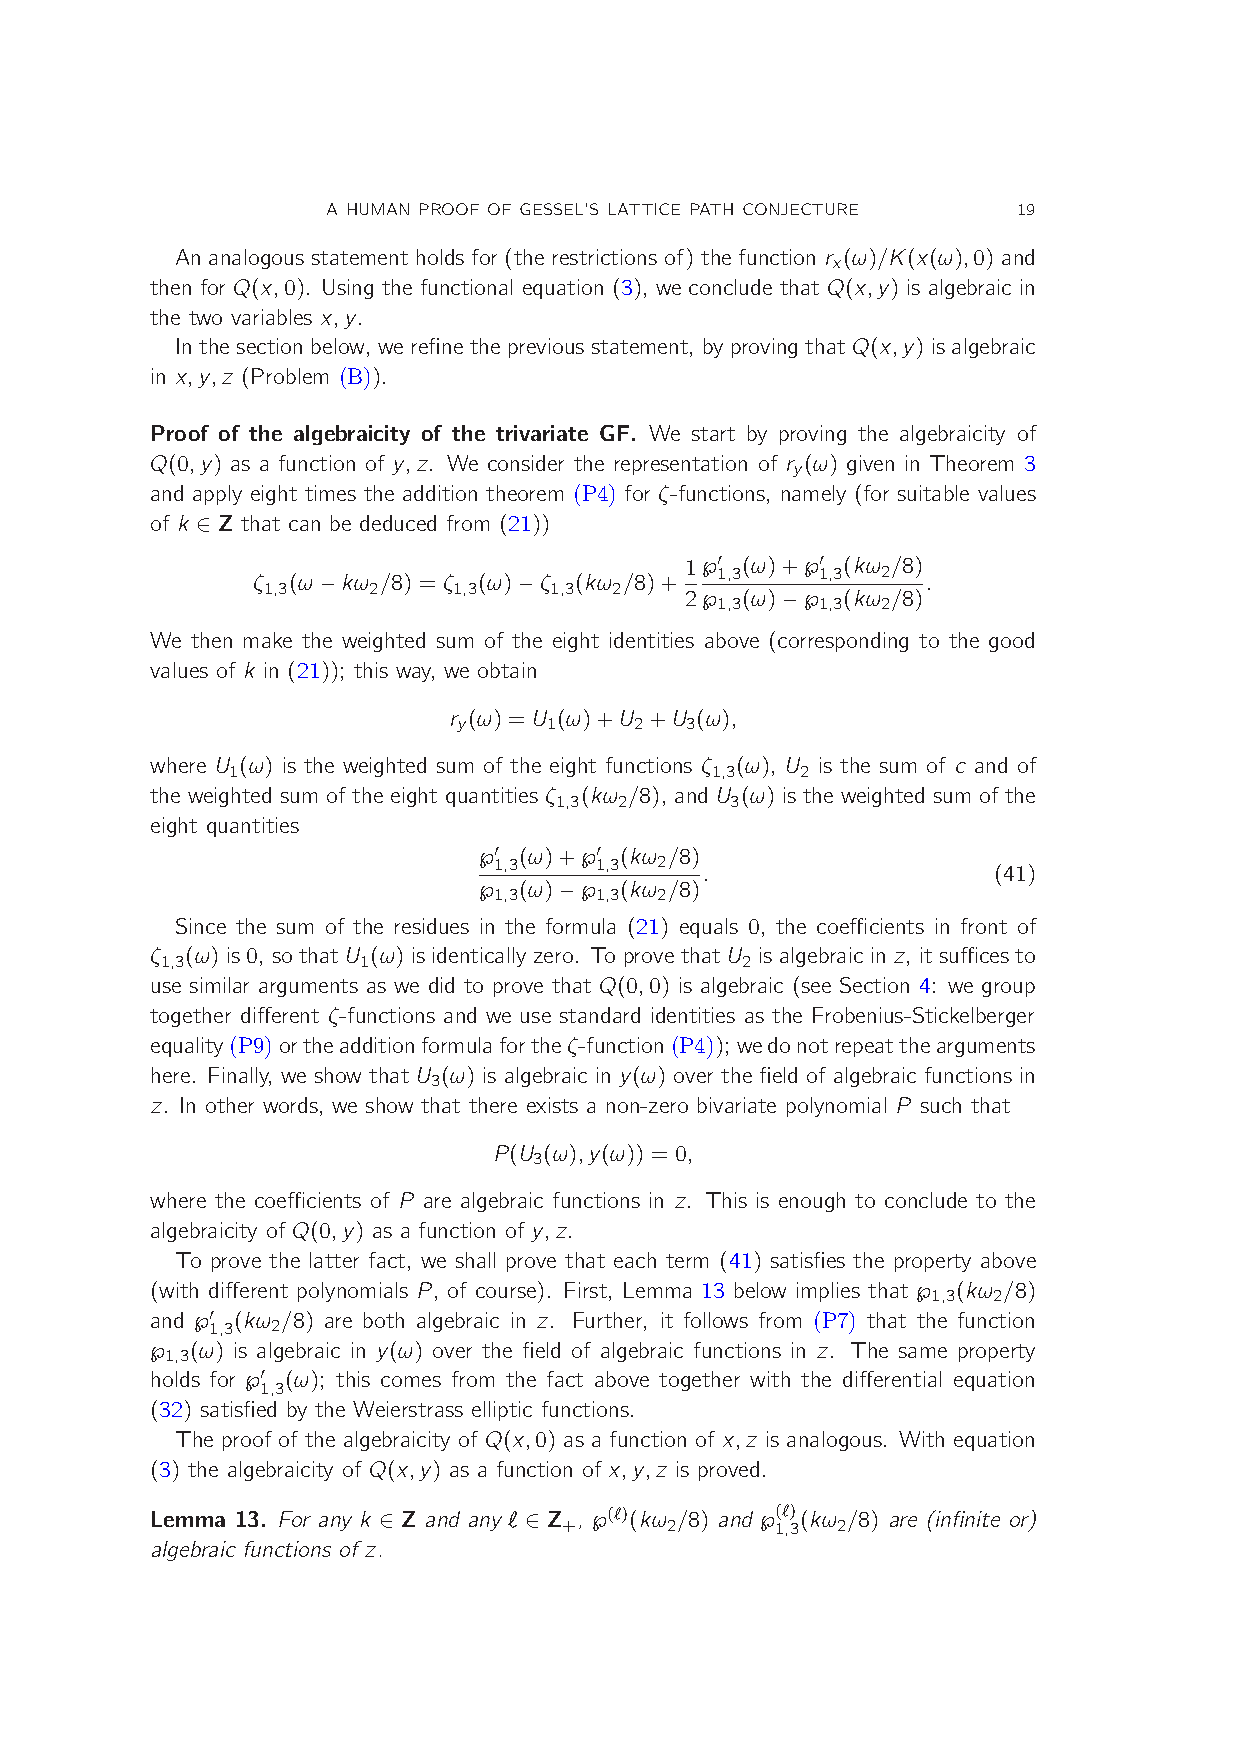
\includegraphics[scale=0.55, clip, trim=0.5cm 17cm 0.5cm 7cm]{HumanProof.pdf}
        \caption{证明一瞥}
      \end{figure}
    }
    \item<5-> 大结局: 在计算机的辅助下被证明, 整个 $3$ 维序列的生成函数 $G(x,y;t)$ 是~\textbf{代数}~的. \cnote{Bostan--Kauers 2010}
    \begin{itemize}
      \item 需要计算前 $n\leq 1200$ 的所有项, 大概 $1.5\times 10^9$ 项.
      \item 求出的最小多项式 $P(G(x, y; t); x, y, t) = 0$ 的系数有 $10^{11}$ 项, 需要 $30~\mathrm{Gb}$ 才能存下!
    \end{itemize}
  \end{itemize}

\end{frame}

\subsection{多元微分有限}

\begin{frame}
  \frametitle{多元整式递推: 如何定义?}

  \begin{itemize}
    \item Zeilberger 最初的尝试: 一个 $f\colon \bbZ_{\geq0}^n \to \bbF$ 的 $n$ 元数列, 对于每个 $1\leq i\leq n$,
    存在一组多项式 $P^{[i]}_j$ ($1\leq j\leq r_i$), 使得满足递推式
    \begin{equation}
      \sum_{j=0}^{r_i} P^{[i]}_j(\bm{m}) f(m_1,\dots,m_i-j,\dots,m_n) = 0.
    \end{equation}
    \pause
    \item 这个定义有严重的问题! Stanley 给出了一个例子: 对于 $f(n, m)(n^2-m) = 0$ 这个方程, 有一组解
    \begin{equation}
      \sum_{n=0}^\infty x^ny^{n^2},
    \end{equation}
    但是这个函数的性质相当复杂, 是我们想要排除的. \cnote{Gessel 90}
  \end{itemize}

\end{frame}

\begin{frame}
  \frametitle{多元微分有限}

  \begin{definition}[多元微分有限]
    一个 $n$ 元生成函数 $F(x_1,\dots,x_n) \in \bbF \llbracket x_1,\dots,x_n \rrbracket$ 是~\textbf{微分有限}~的当且仅当
    \begin{equation}
      \calD F := \Span_{\bbF(x_1,\dots,x_n)} \left\{ \partial_{x_1}^{k_1}\cdots \partial_{x_n}^{k_n} F : \bm{k} \in \bbZ_{\geq 0}^n \right\}
    \end{equation}
    是有限维 $\bbF(x_1,\dots,x_n)$-线性空间.
  \end{definition}
  \begin{itemize}
    \item 等等, 如何赋予 $\bbF \llbracket x_1,\dots,x_n \rrbracket$ 以 $\bbF(x_1,\dots,x_n)$-线性结构?
    (考虑如何展开 $1 / (x - y)$)
    \item 当然嵌入到 $\bbF \llparenthesis x_1 \rrparenthesis\cdots \llparenthesis x_n \rrparenthesis$
    是一种办法, 不过这钦定了一个顺序, 并不典范.
    \item 一个重要的~\textbf{等价定义}: 放宽成对于每个 $1\leq i\leq n$,
    \begin{equation}
      \dim \Span_{\bbF(x_1,\dots,x_n)} \left\{ \partial_{x_i}^k F : k \in \bbZ_{\geq 0} \right\} < \infty
    \end{equation}
  \end{itemize}

\end{frame}

\begin{frame}
  \frametitle{多元微分有限的基本性质}

  \begin{theorem}
    如果 $F, G \in \bbF \llbracket x_1,\dots,x_n \rrbracket$ 是微分有限的, $u_1,\dots,u_n \in \bbF \llbracket t_1,\dots,t_m \rrbracket$ 是代数的,
    那么以下生成函数微分有限:
    \begin{itemize}
      \item $F + G$.
      \item $F\cdot G$.
      \item 良定义的 $F(u_1,\dots,u_n)$.
      \item<2-> \textbf{对角线 \cnote{Lipshitz 1988}}
      \begin{equation}
        \sum_{i_1\dots, i_{n-1} \in \bbZ_{\geq 0}} f_{i_1 \dots i_{n-1} \color{red} i_{n-1}} x_1^{i_1} \cdots x_{n-1}^{i_{n-1}}.
      \end{equation}
    \end{itemize}
  \end{theorem}

\end{frame}

\begin{frame}
  \frametitle{终结比赛的对角线 \cnote{Lipshitz 1988}}

  \begin{itemize}
    \item 几乎所有正常的和式都是微分有限的!
    \begin{equation}
      c_{i,j} = \sum_k a_{i,k} b_{k, j}.
    \end{equation}
    \item<2-> 首先 $A(X, Y)B(Y', Z)$, 然后缩并 $Y$ 和 $Y'$, 然后带入 $Y=1$.
  \end{itemize}

\end{frame}

\begin{frame}
  \frametitle{证明勾勒: 对角线的微分有限性 \cnote{Lipshitz 1988}}

  为了使得呈现更加清晰, 我们只证明二元情况 ($F(x, y)$), 多元情况可以照猫画虎.

  \begin{enumerate}
    \item 换元为 $G = {\color{red}s^{-1}} F(x / s, s)$, 这是关于 $x,s$ ``微分有限''的, 
    不是形式幂级数, 但是仍然满足前述的 $\dim \calD G <\infty$.
    \item 证明存在非零解满足
    \begin{equation}
      \sum_{k, \ell} p_{k,\ell}(x) \partial_x^k \partial_s^\ell G = 0.
    \end{equation}
    \item 设 $o$ 是 $\partial_s^\ell$ 的系数不为零的最小的 $\ell$, 那么上式的 $s^{-o - 1}$ 次项系数给出等式
    \begin{equation}
      \sum_k p_{k, o}(x) \partial_x^k ({\color{red}[s^{-1}]} G) = 0.
    \end{equation}
    \item 说明 $[s^{-1}]G$ 也即 $F$ 的对角线微分有限! \hfill \qedsymbol
  \end{enumerate}

\end{frame}

\begin{frame}
  \frametitle{关键引理 \cnote{Lipshitz 1988}}

  欲证 $\sum_{k, \ell} p_{k,\ell}(x) \partial_x^k \partial_s^\ell G = 0$.
  \begin{itemize}
    \item 根据微分有限性条件, 得到多项式方程 ($\deg L = \ell$)
    \begin{align}
      L(x,s) \partial_x^d G = O(s^d,\partial_x^{d-1}) G,\\
      L(x,s) \partial_s^d G = O(s^d,\partial_s^{d-1}) G.
    \end{align}
    \item 考虑一个大 $N$, 以及所有 $\alpha+\beta\leq N$, 考虑 $L^N \partial_x^\alpha \partial_s^\beta G$,
    通过上述方程不断约化为
    \begin{equation}
      L^N \partial_x^\alpha \partial_s^\beta G = O(s^{(d+\ell)N}, \partial_x^{d-1}, \partial_s^{d-1}) G.
    \end{equation}
    \item 全体 $\alpha, \beta$ 一共有 $\Omega(N^2)$ 种选择, 但右侧的 $s^i \partial_x^j \partial_s^k$
    只有 $\bigO(N)$ 种情况, \textbf{所以当 $\bm N$ 充分大}, 一定可以将左侧 $\bbF(x)$-线性组合得到右侧为 $0$. \hfill \qedhere
    \item 计算这种解的任务一般被称作计算 $\stackrel{\text{syzygy}}{\text{合冲}}$.
  \end{itemize}

\end{frame}

\begin{frame}
  \frametitle{来不及讲的话题}

  \begin{itemize}
    \item 小模数 $p$?
    \begin{itemize}
      \item 固定模数 $p$, 代数幂级数的单项求值都有 ``数位 DP'' 算法.
      \item $p$-自动机和代数幂级数的等价性.
      \item 整式递推除以 $0$?
    \end{itemize}
    \item Weyl 代数 $\bbF[x, \partial]$ 和 Ore 代数 $\bbF[x_1,\dots,x_n, \partial_1,\dots,\partial_n]$?
    \begin{itemize}
      \item 快速计算乘法 (矩阵乘法)?
      \item 不交换的代数结构, 但是可以定义一个方向的 Euclid 算法和 gcd.
    \end{itemize}
    \item $q$-整式递推?
    \begin{itemize}
      \item 咬文嚼字: [二项式 / 整式递推 / 超几何级数 / ...] 的 $\stackrel{q\text{-analog}}{q\text{-类比}}$,
      或者 $q$-[二项式 / 整式递推 / 超几何级数 / ...],
      而不是单独说 ``$q$-类比''?
    \end{itemize}
  \end{itemize}

  \bigskip

  \begin{center}
    ``还有许多问题我愿意告诉你们, 但是你们现在尚不能接受.''

    \hfill --- A.~Кострикин, 代数学引论
  \end{center}

\end{frame}

\begin{frame}
  \frametitle{延伸阅读}

  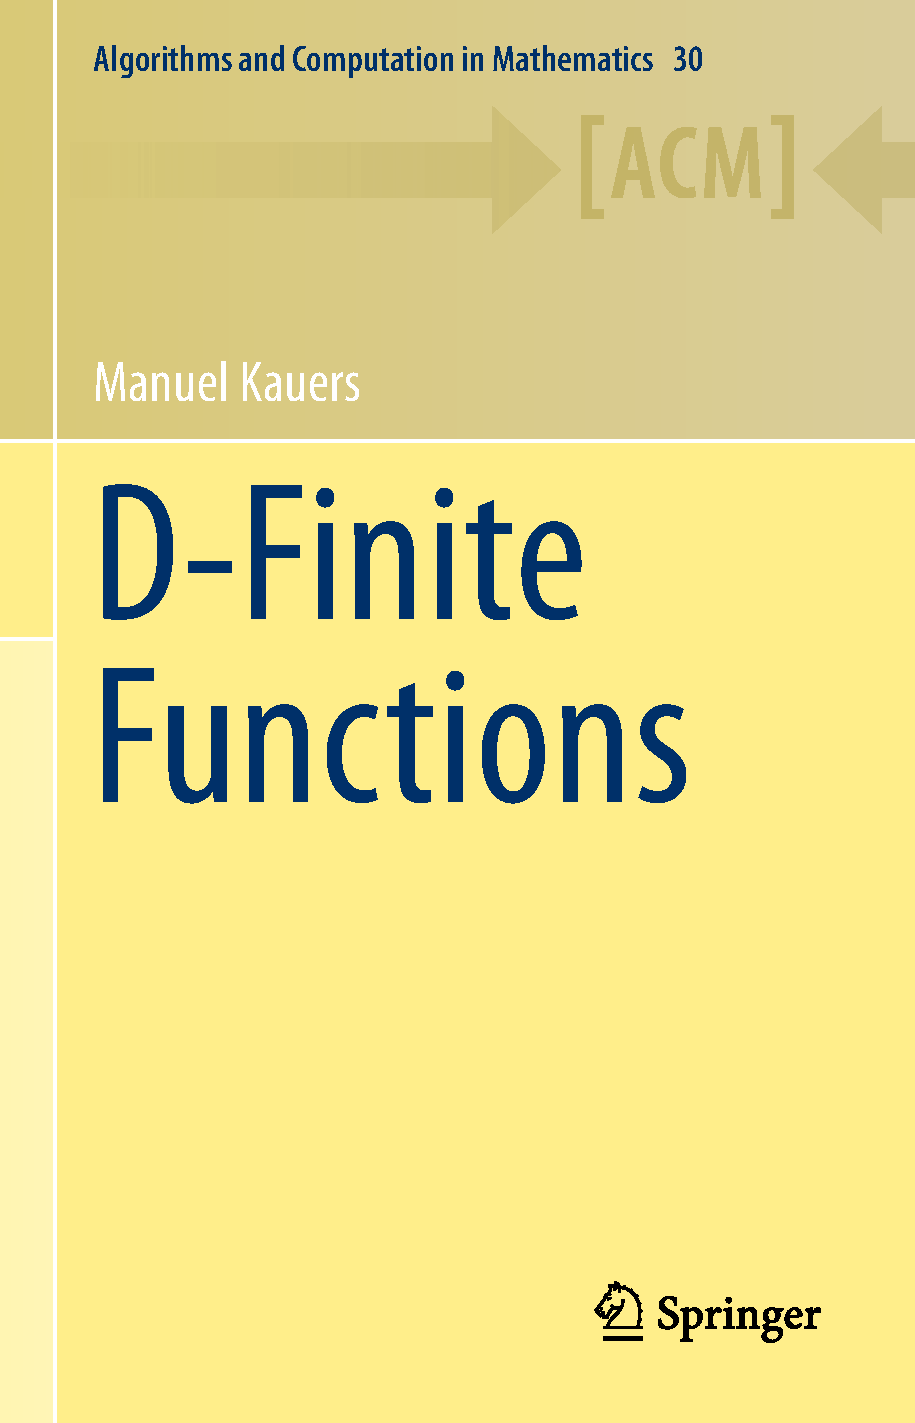
\includegraphics[scale=0.2]{DFinite.pdf}
  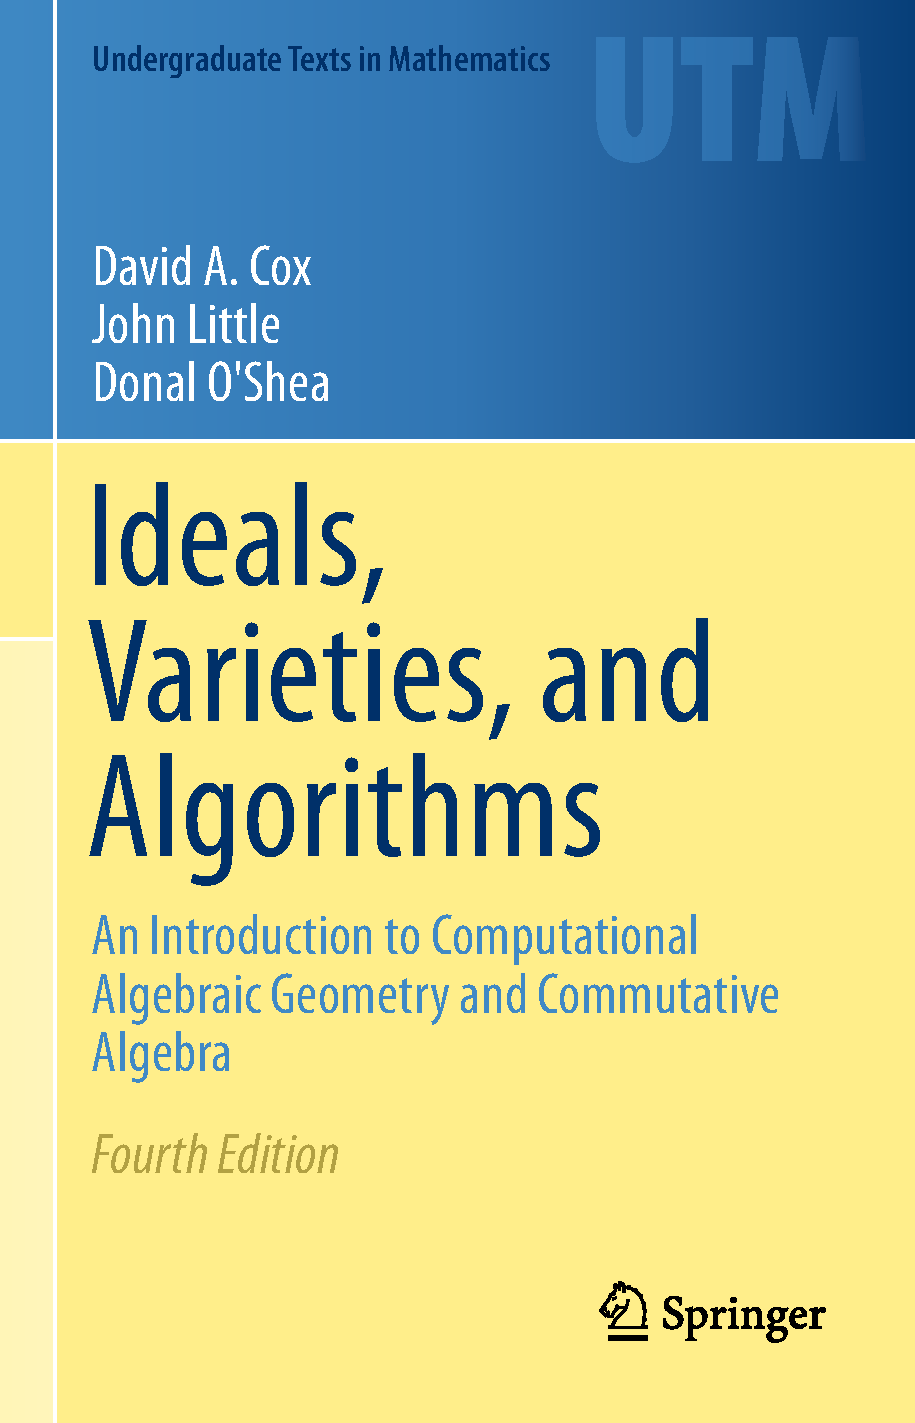
\includegraphics[scale=0.2]{AG.pdf}
  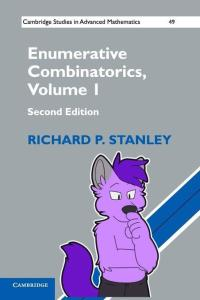
\includegraphics[scale=0.45]{EC.jpeg}

\end{frame}

\subsection{整式递推在 OI 中的未来}

\begin{frame}
  \frametitle{后日谈: 整式递推在 OI 中的未来}

  \begin{itemize}
    \item<1-> ``很多序列都是整式递推的'', 这是一个对于我们理解问题的正面消息, 同时也是对出题人的新考验.
    \item<2-> 出题人: 我动用了很多智慧, 最后得到了这个问题答案的递推式!
    \item<3-> 选手: 跑几项暴力, Min25 BM 直接秒了, 真简单!
    \item<4-> 出题人: 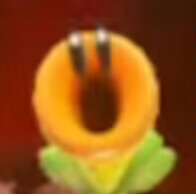
\includegraphics[scale=0.2]{woc.jpg}
  \end{itemize}

\end{frame}

\begin{frame}
  没有绝对的``最小递推式'', 只有 Pareto 最优!
  \begin{figure}
    \centering
    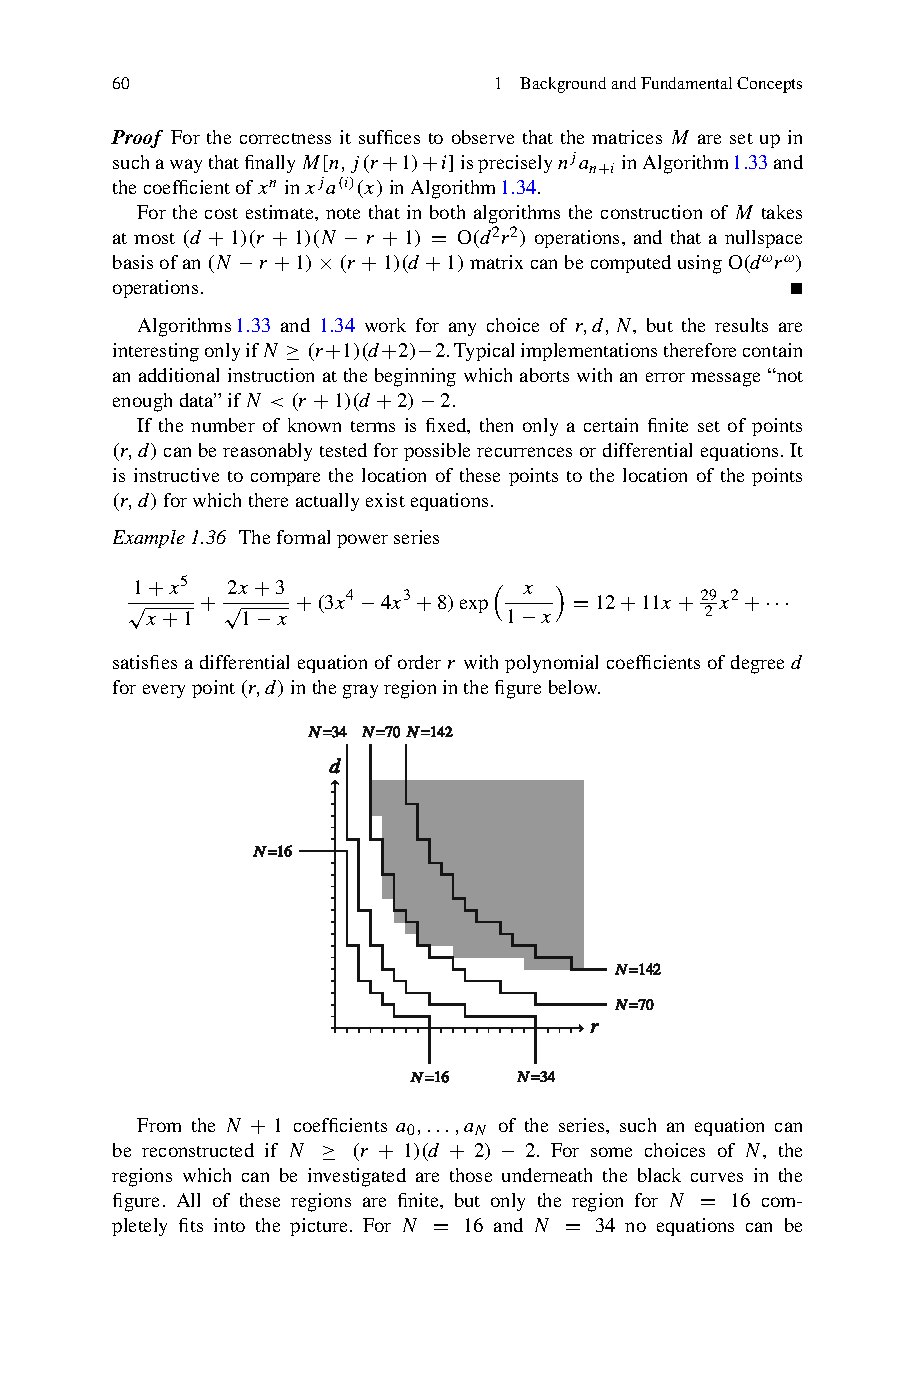
\includegraphics[scale=0.7, clip, trim=0.5cm 5cm 0.5cm 8.8cm]{Kauers.pdf}
    \caption{递推式的长度--多项式次数的权衡 \cnote{Kauers 2023}}
  \end{figure}

\end{frame}

\begin{frame}
  \frametitle{没有一劳永逸的方法}

  \begin{itemize}
    \item<1-> 微分有限这一定义本身并不能完整捕捉 $\stackrel{\text{effective}}{\text{有效}}$ 的递推式.
    \item<2-> 回归一个古老的启蒙问题: 给定多项式 $f(x)$, 求出 $f(x)^n$ 的各项系数.
    \begin{itemize}
      \item<3-> 记 $g(x) = f(x)^n$, 那么可以利用 $g'f = nf'g$ 来递推.
      \item<4-> 如果 $f(x)$ 不是低次多项式, 而是~\textbf{稀疏多项式}, 方法仍然奏效, 但难以用 Min25 BM 解决.
      \item<5-> \textbf{稀疏整式递推}, 需要理解操作原理才能得到~\textbf{有效}~递推式的问题.
    \end{itemize}
    \item<6-> \textbf{隐式整式递推}: 答案序列 $f(n)$ 本身并非整式递推, 但是计算某一项的时候具有整式递推的内核.
    \begin{itemize}
      \item<7-> 截取--Taylor--截取: $\bigO(n)$ 计算 Bernoulli 数 $B_n = [x^n / n!] \frac{x}{\exp x - 1}$.
      \item<8-> 思考题: $\widetilde \bigO(n)$ 计算 $n$ 个顶点的, \textbf{不存在}~$2$ 度点的图的数量.
    \end{itemize}
    \item<9-> 相信大家的智慧!
  \end{itemize}

\end{frame}

\frame
{
  \centering 
  {\Large 感谢倾听}

  \bigskip

  {\kaishu ``此时相望不相闻, 愿逐月华流照君.''}

  \vspace{\fill}

  {\footnotesize 感谢: $\stackrel{\textbf{PinkRabbit}}{\text{陈亮舟}}$, 任舍予,
  $\stackrel{\textbf{sys.}}{\text{史钰申}}$, $\stackrel{\textbf{ix35}}{\text{万成章}}$,
  $\stackrel{\textbf{he\_\_\_\_\_he}}{\text{许庭强}}$,
  $\stackrel{\textbf{yyc 樱初音}}{\text{杨亦诚}}$,
  $\stackrel{\textbf{negiizhao}}{\text{赵雨扬}}$\footnote{按照字典顺序排列.} 协助我准备本次报告.}
}

\end{document}
